\documentclass[a4paper, 12pt]{article}
\usepackage[utf8]{inputenc}
\renewcommand\familydefault{\sfdefault}
\usepackage[T1]{fontenc}
\usepackage[francais]{babel}
\usepackage[left=2.5cm,top=2.5cm,right=2.5cm,bottom=2.5cm]{geometry}
\usepackage[onehalfspacing]{setspace}
\usepackage{graphicx}
\usepackage[usenames, dvipsnames]{xcolor}
\definecolor{mygray}{gray}{0.95}

\usepackage{minted}
\usemintedstyle{colorful}
\usepackage{float}
\floatplacement{figure}{H}
\usepackage{authblk}
\usepackage{enumitem}
\setlist[enumerate]{label*=\arabic*.}
\usepackage{hyperref}
\hypersetup{
    colorlinks,
    citecolor=black,
    filecolor=black,
    linkcolor=black,
    urlcolor=blue
}

\usepackage{caption}
\newenvironment{code}{\captionsetup{type=listing}}{}
\usepackage{array}
\usepackage{etoolbox}
\patchcmd{\thebibliography}{\section*{\refname}}{}{}{}

\usepackage{dirtree}
\usepackage{tabularx}

\usepackage{glossaries}
	\let\oldnewacronym\newacronym
	\newcommand*{\provideacronym}[3]{%
	  \ifglsentryexists{#1}{%
	  }{%
	    \oldnewacronym{#1}{#2}{#3}%
	  }%
	}
\makeglossaries

\usepackage{fancyhdr}
\pagestyle{fancy}
\fancyhf{}
\lhead{Movies App}
\rhead{\leftmark}
\lfoot{Jeremy Favre - Steven Liatti}
\rfoot{\thepage}
\renewcommand{\footrulewidth}{1pt}

\usepackage{pdfpages}

\begin{document}

\title{Movies App}
\author{Jeremy Favre - Steven Liatti}
\date{Janvier 2020}
\maketitle
\begin{figure}
    \begin{center}
        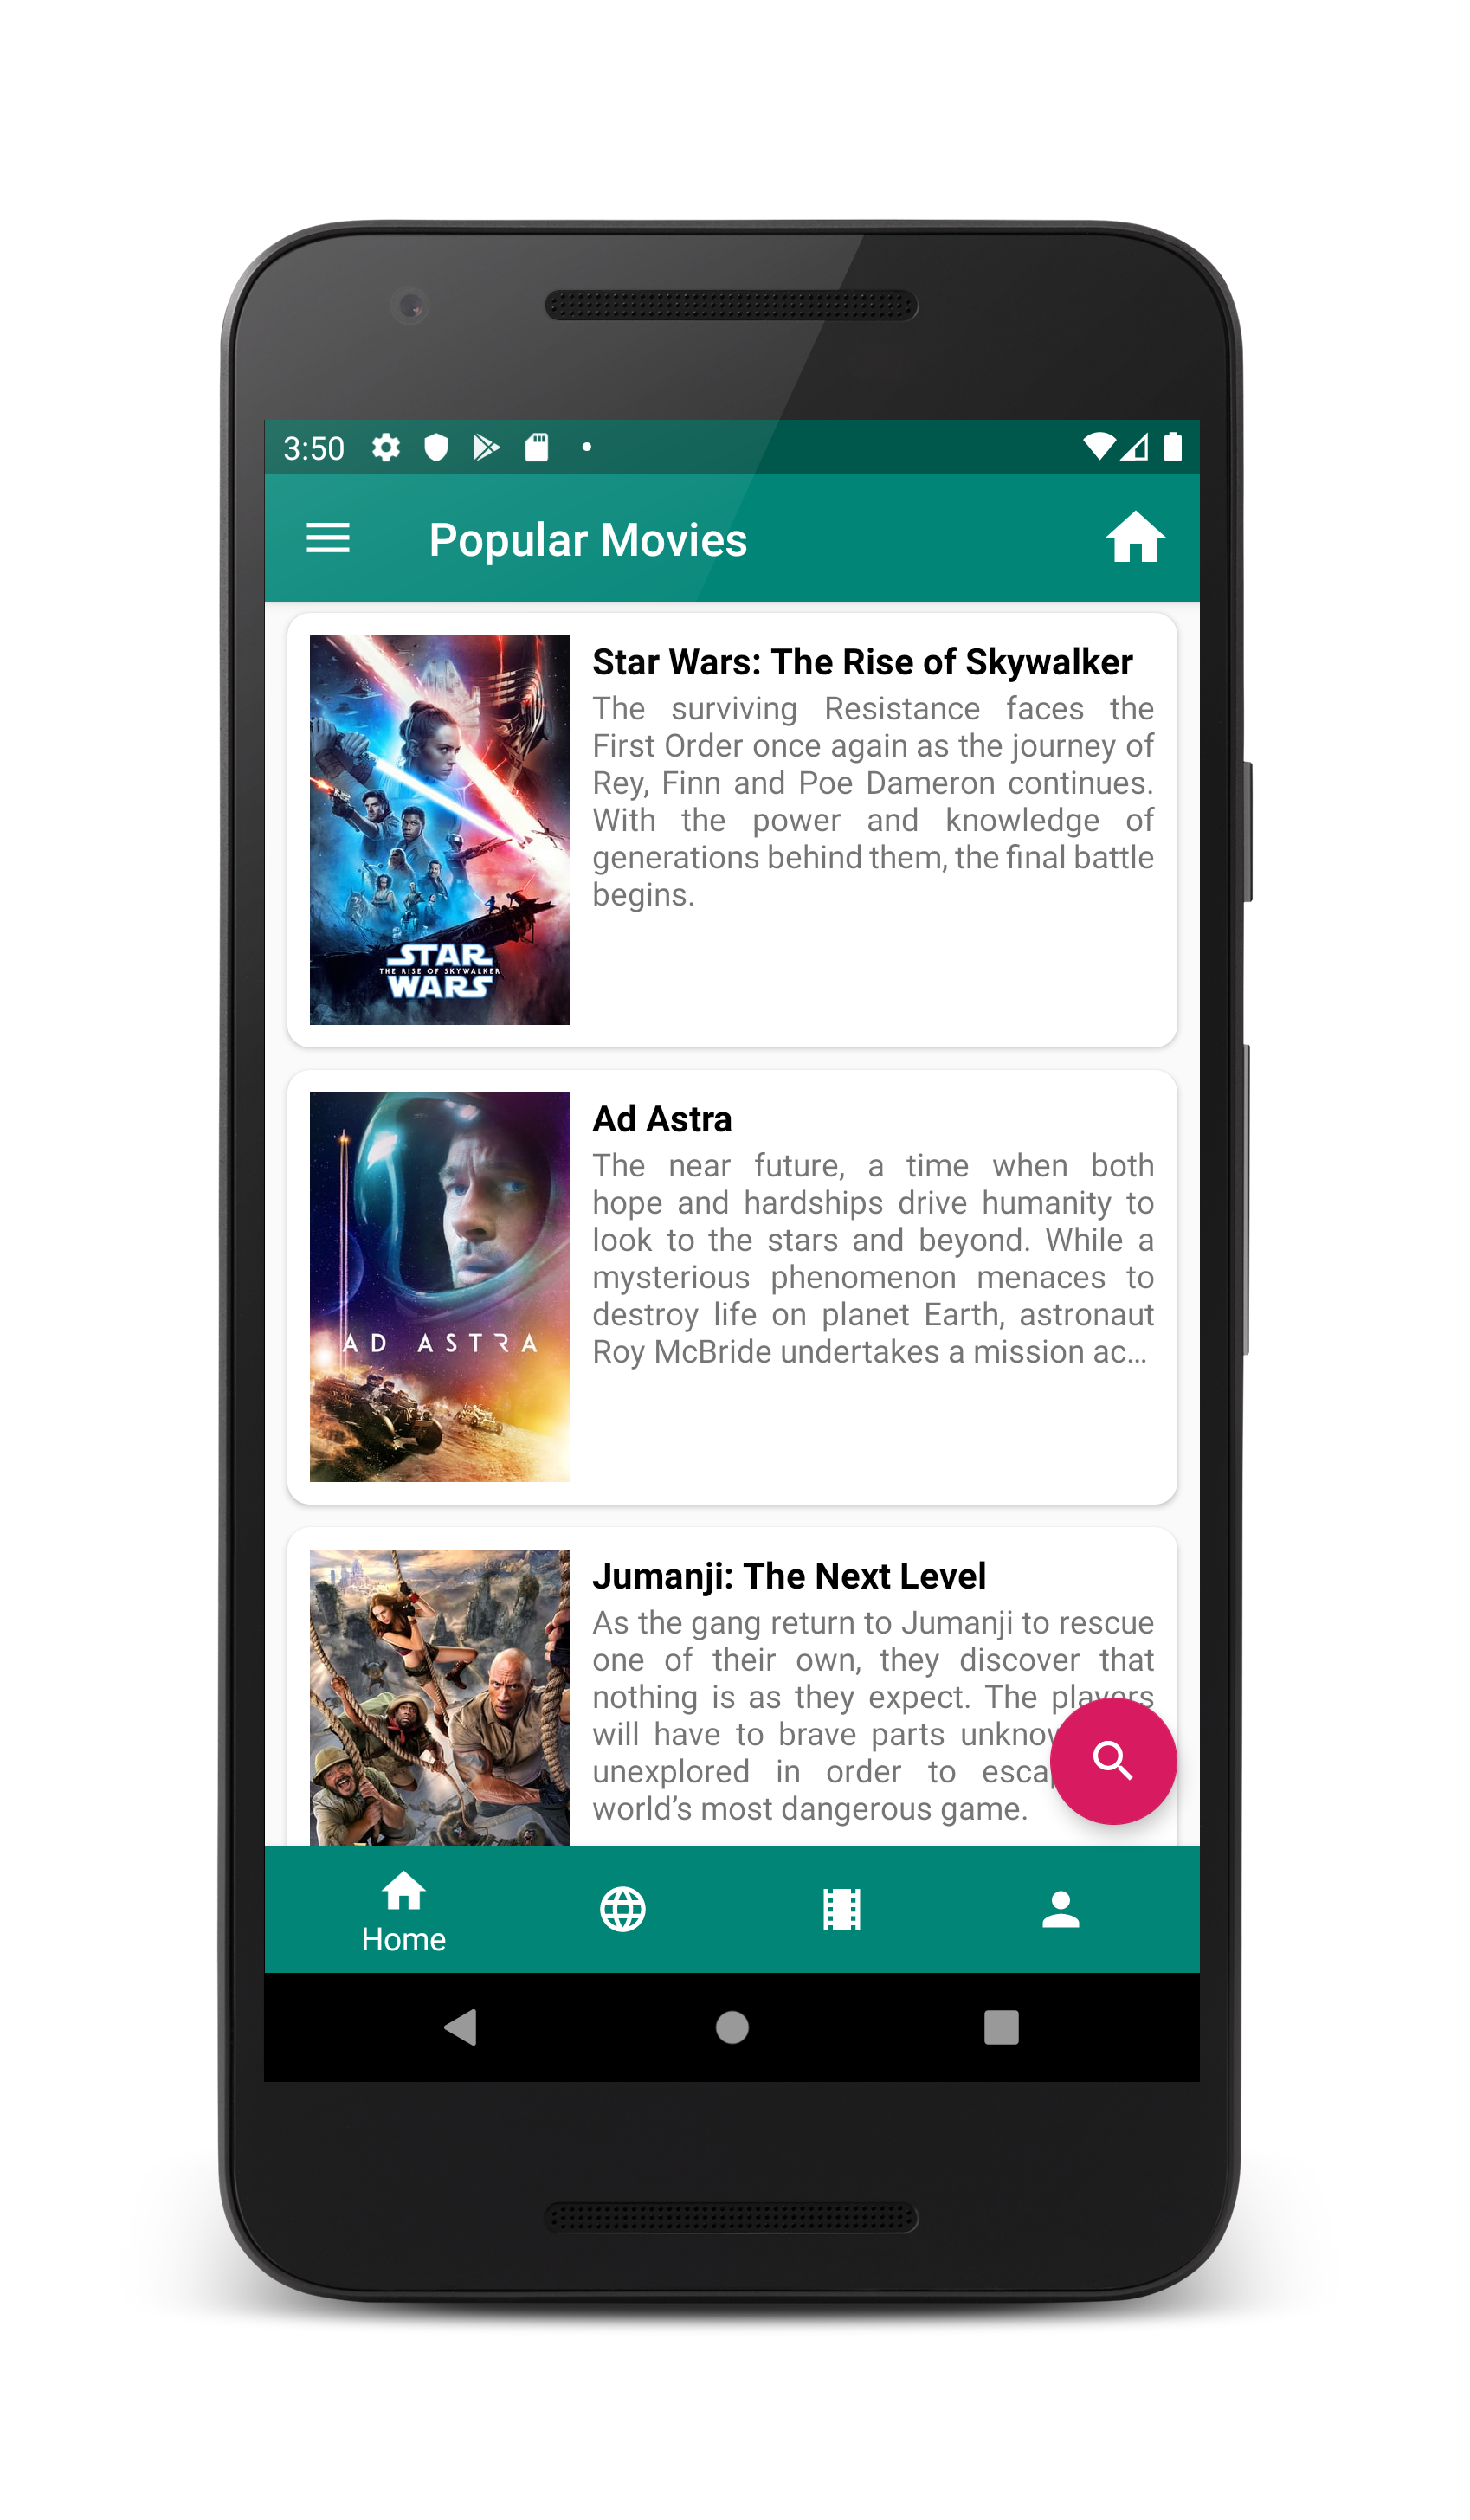
\includegraphics[width=0.65\textwidth]{img/screenshots/movie_list_framed.png}
    \end{center}
\end{figure}
\newpage


% \setcounter{tocdepth}{2}
\addcontentsline{toc}{subsection}{Table des matières}
\tableofcontents
\addcontentsline{toc}{subsection}{Table des figures}
\listoffigures
% \renewcommand{\listtablename}{Table des tables}
% \addcontentsline{toc}{subsection}{Table des tables}
% \listoftables
% \newpage
\renewcommand\listoflistingscaption{Table des listings de code source}
\addcontentsline{toc}{subsection}{Table des listings de code source}
\listoflistings

\subsection*{Conventions typographiques} %-----------------------------------------------------------------------------------------------
\addcontentsline{toc}{subsection}{Conventions typographiques}
Lors de la rédaction de ce document, les conventions typographiques ci-dessous ont
été adoptées.
\begin{itemize}[label=\textbullet]
	\item Tous les mots empruntés à la langue anglaise ou latine ont été écrits en \textit{italique}.
	\item Toute référence à un nom de fichier (ou répertoire), un chemin d'accès, une 
    utilisation de paramètre, variable, commande utilisable par l'utilisateur, ou extrait de code 
    source est écrite avec une police d'écriture à \mintinline{text}{chasse fixe}.
	\item Tout extrait de fichier ou de code est écrit selon le format suivant:
    \bigbreak
    \begin{code}
        \begin{minted}[bgcolor=mygray,breaklines,breaksymbol=,linenos,frame=single,stepnumber=1,tabsize=2]{kotlin}
fun main() {
    println("Hello World!")
}
        \end{minted}
    \end{code}
    \item Dans les listings, les lignes précédées d'un "\$" sont exécutées dans un shell.
\end{itemize}


\newacronym{api}{API}{\textit{Application Programming Interface}, Interface de programmation : services offerts par un programme producteur à d'autres programmes consommateurs}
\newacronym{json}{JSON}{\textit{JavaScript Object Notation}, Format d'échange de données léger, facile à lire et écrire par les humains et les machines}
\newacronym{xml}{XML}{\textit{Extensible Markup Language}, Langage extensible de description de données}
\newacronym{jvm}{JVM}{\textit{Java Virtual Machine}, Exécute le bytecode Java sur différents systèmes d'exploitation}
\printglossary[type=\acronymtype,title={Acronymes}]
\newpage


\section{Introduction} %-----------------------------------------------------------------------------------------------

\subsection{Buts}
De nos jours, les médias sont à la portée de tous et accessibles très facilement notamment grâce aux plateformes telle que Netflix, streaming et bien d'autres encore. Il est donc difficle d'effectuer un choix parmi ces milliers de films mis à disposition. C'est là qu'entre en jeu notre mini-projet que nous avons réalisé dans le cadre du cours de Systèmes d'exploitation mobiles et applications. L'objectif est de développer une application dediée à la plateforme Android qui propose à ses utilisateurs divers services, tels que la liste des films à la une, obtenir les films similaires à un film, les acteurs concernés et la possibilité de rechercher un film en particulier.
2019 oblige, un aspect social est également présent au sein de cette application, l'utilisateur pourra renseigner son appréciation personnelle à propos d'un film, mais également de pouvoir suivre d'autres utilisateurs afin de connaitre leurs appréciations sur différents films qu'ils ont visionnés.
La forme "nous" est utilisée tout au long de ce rapport étant donné que ce projet est réalisé par binôme.

\subsection{Motivations}
Le périmètre de ce projet semblait parfaitement adapté pour exploiter la majorité des techniques et méthodes vues durant le cours de développement d'application mobiles.
Ce projet est une formidable occasion pour relier la mise en pratique des connaissances acquises en cours et notre passion cinéphile commune. Nous sommes également convaincus que notre entourage (ou un réseau plus large) se servirait volontiers d'une telle application.

\subsection{Méthodologie de travail}
Sur la base d'une analyse préliminaire, nous avons séparé le travail en plusieurs tâches que nous avons assigné à chaque membre du binôme de manière équitable afin d'effectuer le travail en parallèle.
Nous avons adopté une pseudo méthode "agile", en factorisant le projet en petites tâches distinctes et en nous fixant des délais pour les réaliser. Le partage du code s'est fait avec git et gitlab. Nous nous sommes servis des \textit{issues} gitlab pour représenter nos tâches et du "board" du projet pour avoir une vision globale du travail accompli (par qui et quand) et du travail restant.

\newpage

\section{Conception et analyse} %-----------------------------------------------------------------------------------------------
Nous avons commencé par dessiner les maquettes des vues de notre application afin de se faire une idée de l'aspect visuel de chaque vue et des relations entre elles, comme illustré à la figure \ref{maquettes}. Tout cela dans le but de simplifier et clarifier la phase de développement proprement dite.
Durant cette phase, nous nous sommes également documentés sur les \acrshort{api}s existantes proposant des services relatifs aux films, nous avons étudié les différentes technologies permettant de mettre en place une \acrshort{api} REST et finalement nous avons analysé les composants et méthodologies étudiés en cours qui seraient utiles d'intégrer dans notre application.
Les sous-sections suivantes décrivent les vues et les fonctionnalités que propose l'application finale.

\subsection{Films tendance}\label{films-tendance}
Lorsqu'un utilisateur ouvre l'application, la vue principale (home) lui affiche une liste des films à la une, classés en fonction de leur popularité. Chaque film affiche ses informations de base (poster, titre, courte description). L'utilisateur a la possibilité de cliquer sur un film afin d'obtenir d'avantage d'informations.

\subsection{Détails d'un film}
Comme décrit à la section \ref{films-tendance}, si l'utilisateur souhaite en savoir plus sur un film, il peut accéder à cette vue présentant les détails d'un film. Elle comporte les informations détaillées du film tel que le titre, la description complète, la liste des acteurs, la liste des réalisateurs, les différentes bande-annonces, les genres associés et une grille qui contient les films similaires au film concerné. La possibilité de cliquer sur un film de la grille afin de naviguer vers ses détails est également intégrée.
Si l'utilisateur souhaite visionner une bande-annonce, il lui suffit de cliquer dessus afin que le \textit{player} YouTube soit automatiquement lancé avec la vidéo en question.
C'est également depuis cette vue qu'il pourra indiquer son appréciation pour le film ("like" ou "dislike"), appréciation qui sera sauvegardée dans son profil.

\begin{figure}
    \begin{center}
        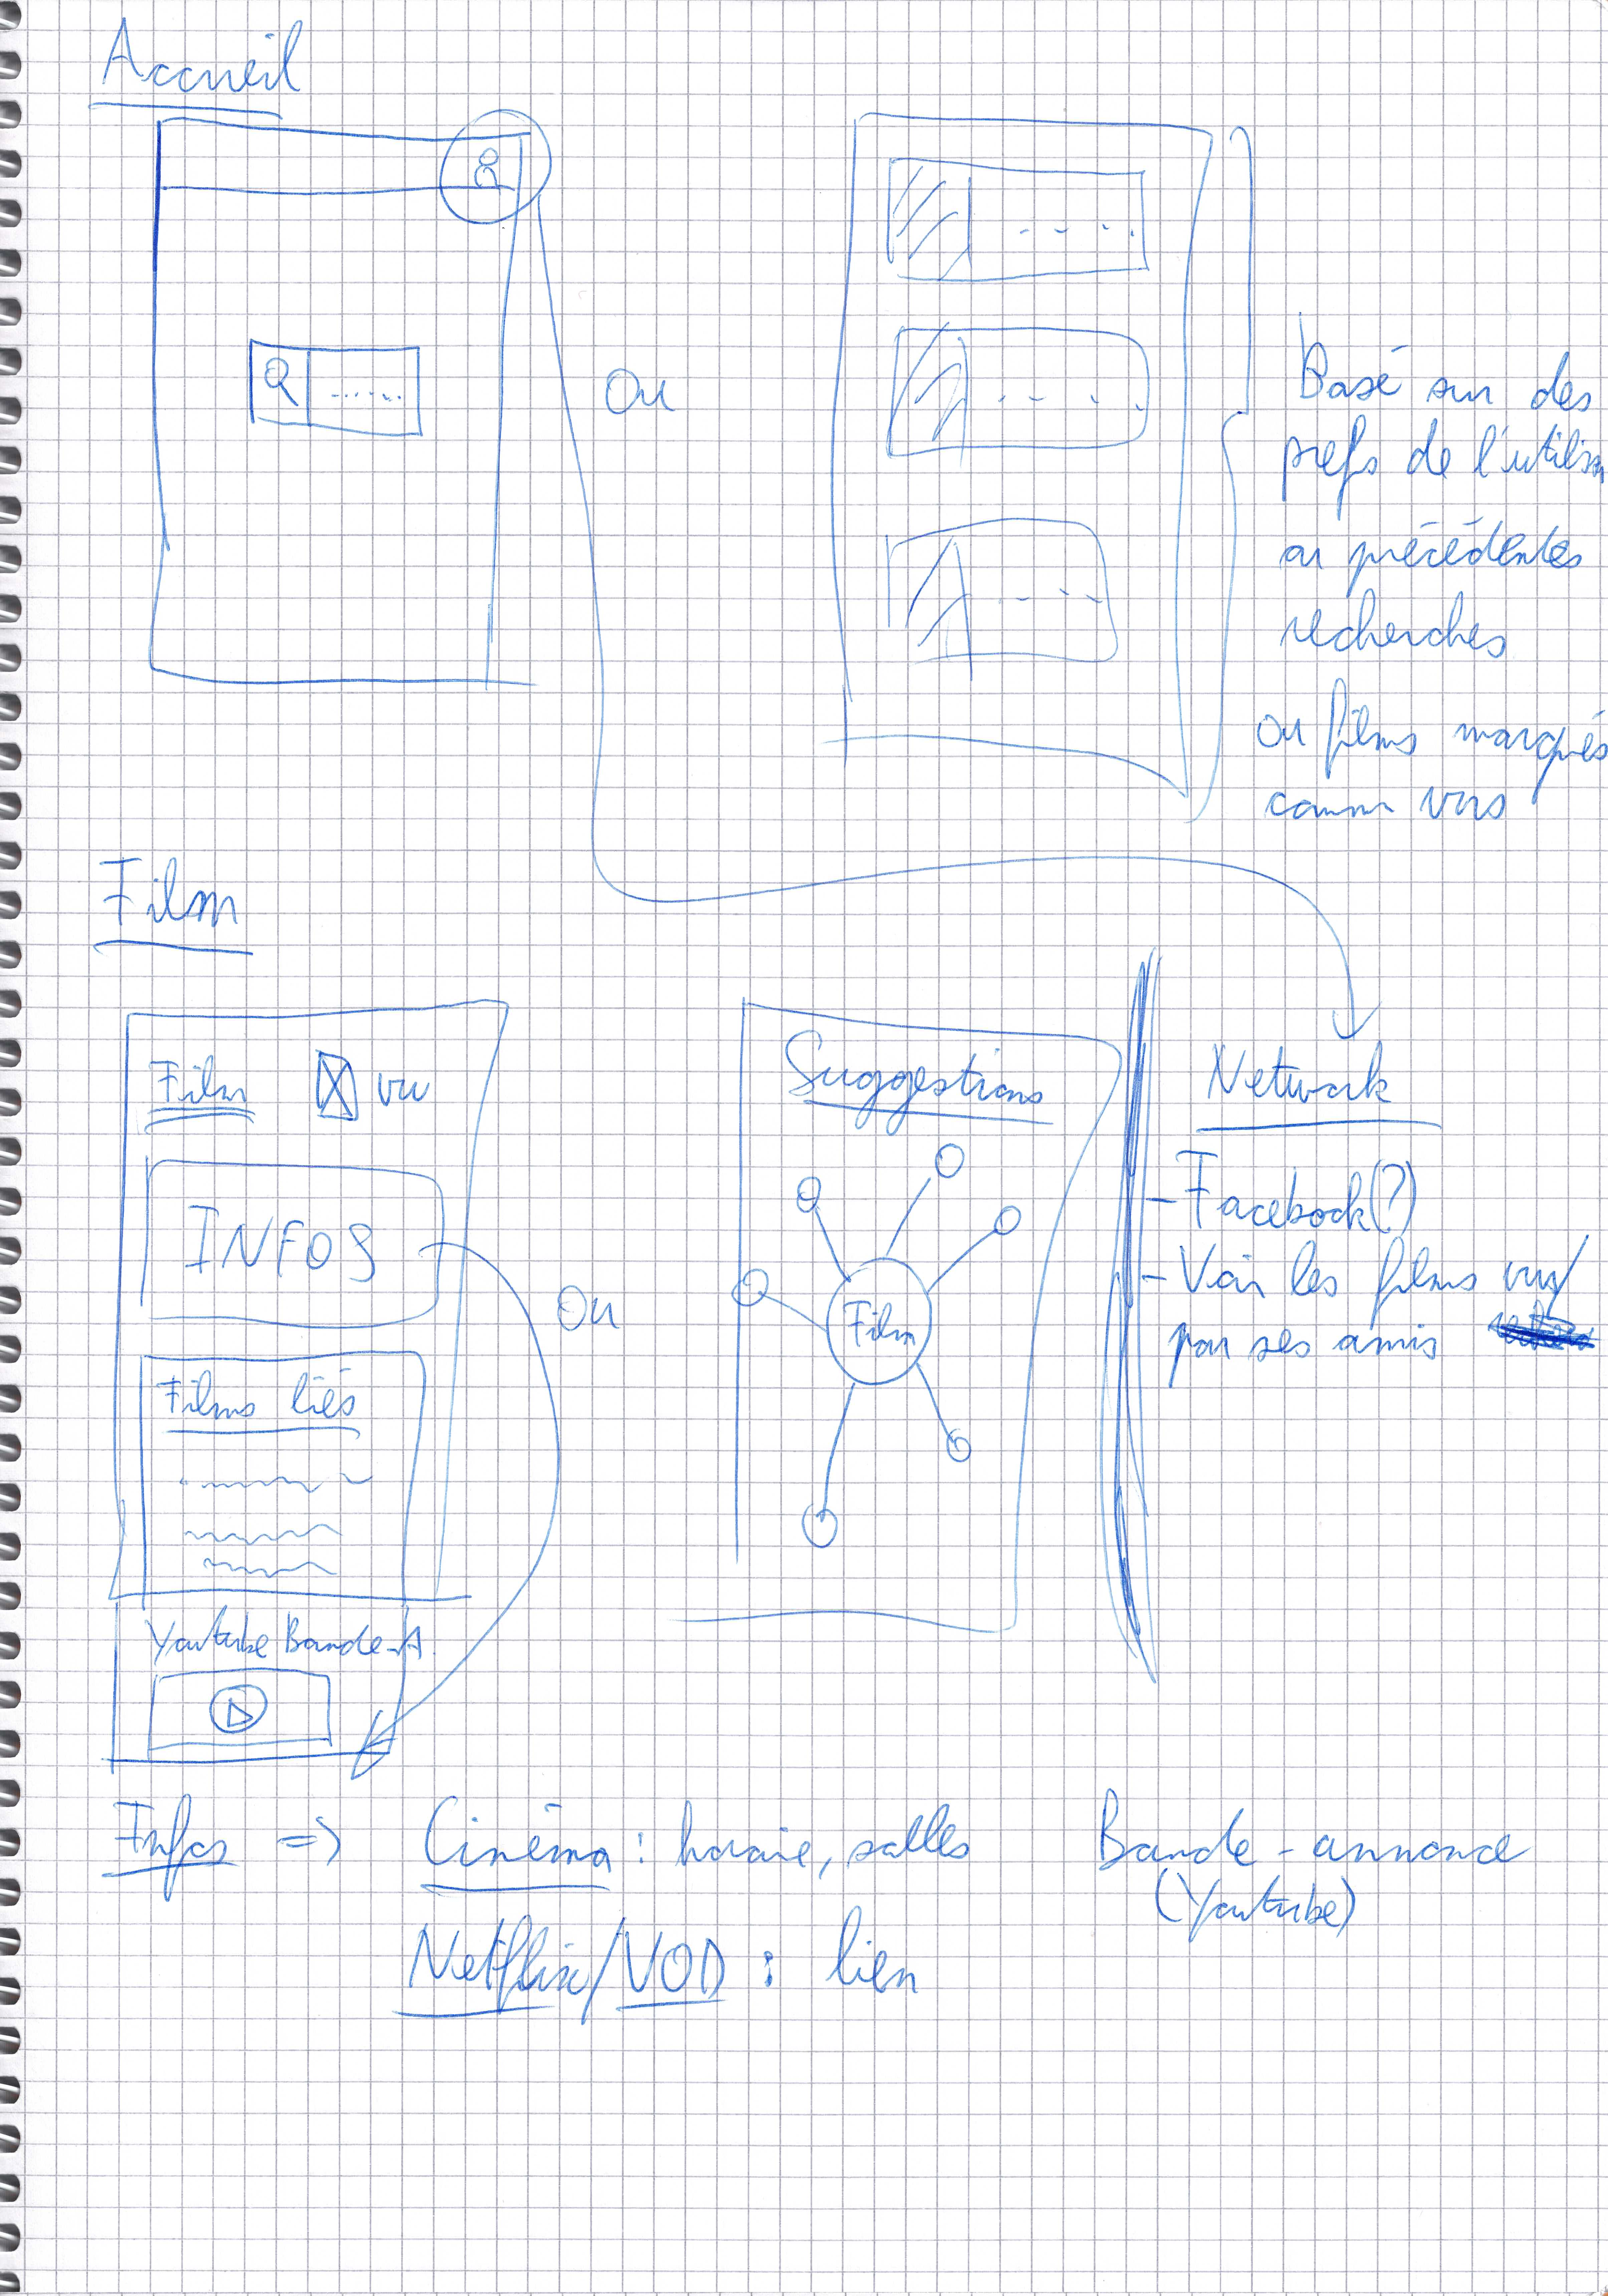
\includegraphics[width=0.8\textwidth]{img/maquettes.jpg}
    \end{center}
    \caption{Maquettes à main levée des vue de l'application}
    \label{maquettes}
\end{figure}

\subsection{Recherche}
Une interface de recherche est mise à disposition. La recherche peut être lancée parmi les films, les acteurs ou les autres utilisateur de l'application selon le choix de l'utilisateur (bouton "radio" ou mécanisme similaire).
Les résultats de la recherche seront présentés sous forme de liste, présentant les différentes actions selon le type de recherche qui aura été effectué :
\begin{itemize}
    \item Si l'utilisateur cherche un film, il obtiendra la liste des films qui correspondent aux critères entrés dans le champs texte de recherche.
    \item S'il cherche un acteur, il obtiendra une liste d'acteurs avec la possibilité de cliquer dessus (comme pour les films) afin d'afficher plus de détails à leur sujet.
    \item S'il cherche un autre utilisateur, il aura alors la possibilité de le suivre en l'ajoutant à son réseau d'amis.
\end{itemize}

\subsection{"Peoples"}
Au même titre que la liste des films tendance, nous avons une interface proposant la liste des acteurs actuellement populaires avec la possibilité de cliquer sur chacun d'entre eux afin d'obtenir plus d'informations à leur sujet.

\subsection{Détails d'un "people"}
Comme pour les détails d'un film, nous avons également une vue présentant les détails d'un acteur, elle permet de consulter diverses informations, telles que sa biographie personnelle et la liste des films dans lesquels il a joué.

\subsection{Mes films}\label{mes-films}
Si l'utilisateur possède un compte dans l'application, il pourra retrouver sa liste de films appréciés ou non, sous une forme similaire à la liste des films tendance (sous-section \ref{films-tendance}).

\subsection{Réseau d'amis}\label{reseau-amis}
La vue réseau d'amis est disponible uniquement si l'utilisateur détient un compte. Son réseau d'amis sera constitué d'une liste d'utilisateurs le suivant (ses "\textit{followers}") ainsi que d'une liste d'utilisateurs auxquels il est abonné (ses "\textit{following}").

\subsection{Authentification}
Au sein de l'application, l'authentification est requise pour consulter certaines vues spécifiques, comme le réseau d'amis (\ref{reseau-amis}) ou les films préférés (\ref{mes-films}) et les vues comprenant des éventuelles informations persistées.
Les autres vues de l'application ne requièrent aucune authentificaion. Ce principe a été mis en place afin de ne pas reproduire un des principaux points faibles des applications actuelles qui est de forcer l'utilisateur à s'authentifier sous peine de ne pas pouvoir utiliser l'application. Notre application demandera à l'utilisateur de s'authentifier uniquement lorsque cela est nécessaire.
 
\subsubsection{Connexion}
La vue connexion comporte simplement deux champs permettant de renseigner le pseudo et le mot de passe afin de s'authentifier.

\subsubsection{Enregistrement}
Cette vue comporte les champs nécessaires à la création d'un compte, à savoir un pseudo (unique), un email et un mot de passe.

\subsection{Navigation}
Pour naviguer d'une vue à une autre, l'utilisateur dispose de différents mécanismes.

\subsubsection{Tabs de navigation}
En bas de l'écran, nous retrouvons une liste de \textit{tabs} (onglets) permettant de naviguer entre les différentes vues de l'application.

\subsubsection{Barre de navigation}
En haut de l'écran se trouve une barre comportant le nom de la vue courrante, un bouton "home" (\ref{films-tendance}) et un contrôle faisant apparaitre le menu latéral.

\subsubsection{Menu latéral}
Finalement, nous avons un menu latéral qui apparaît de gauche à droite de l'écran. Ce menu permet d'afficher les informations relatives au profil de l'utilisateur courant. D'autre part, il propose les action de connexion, création de compte et déconnexion. Si l'utilisateur est connecté, il pourra aussi naviguer vers les vues des films aimés et du réseau d'amis.

\newpage

\section{Implémentation} %-----------------------------------------------------------------------------------------------
Dans cette partie concernant l'implémentation, nous allons présenter les différentes technologies, méthodes et composants utilisés afin de mener à bien le développement de notre application. Des captures d'écran illustreront le résultat final.

% TODO: screen des fichiers
\subsection{Structure du projet et arborescence des fichiers}

\subsection{APIs}
Pour échanger les informations requises, notre application interagit avec des \acrshort{api}s externes permettant d'obtenir et persister les données nécessaires aux différentes fonctionnalités proposées, comme illustré à la figure \ref{apis_usage}.
\begin{figure}
    \begin{center}
        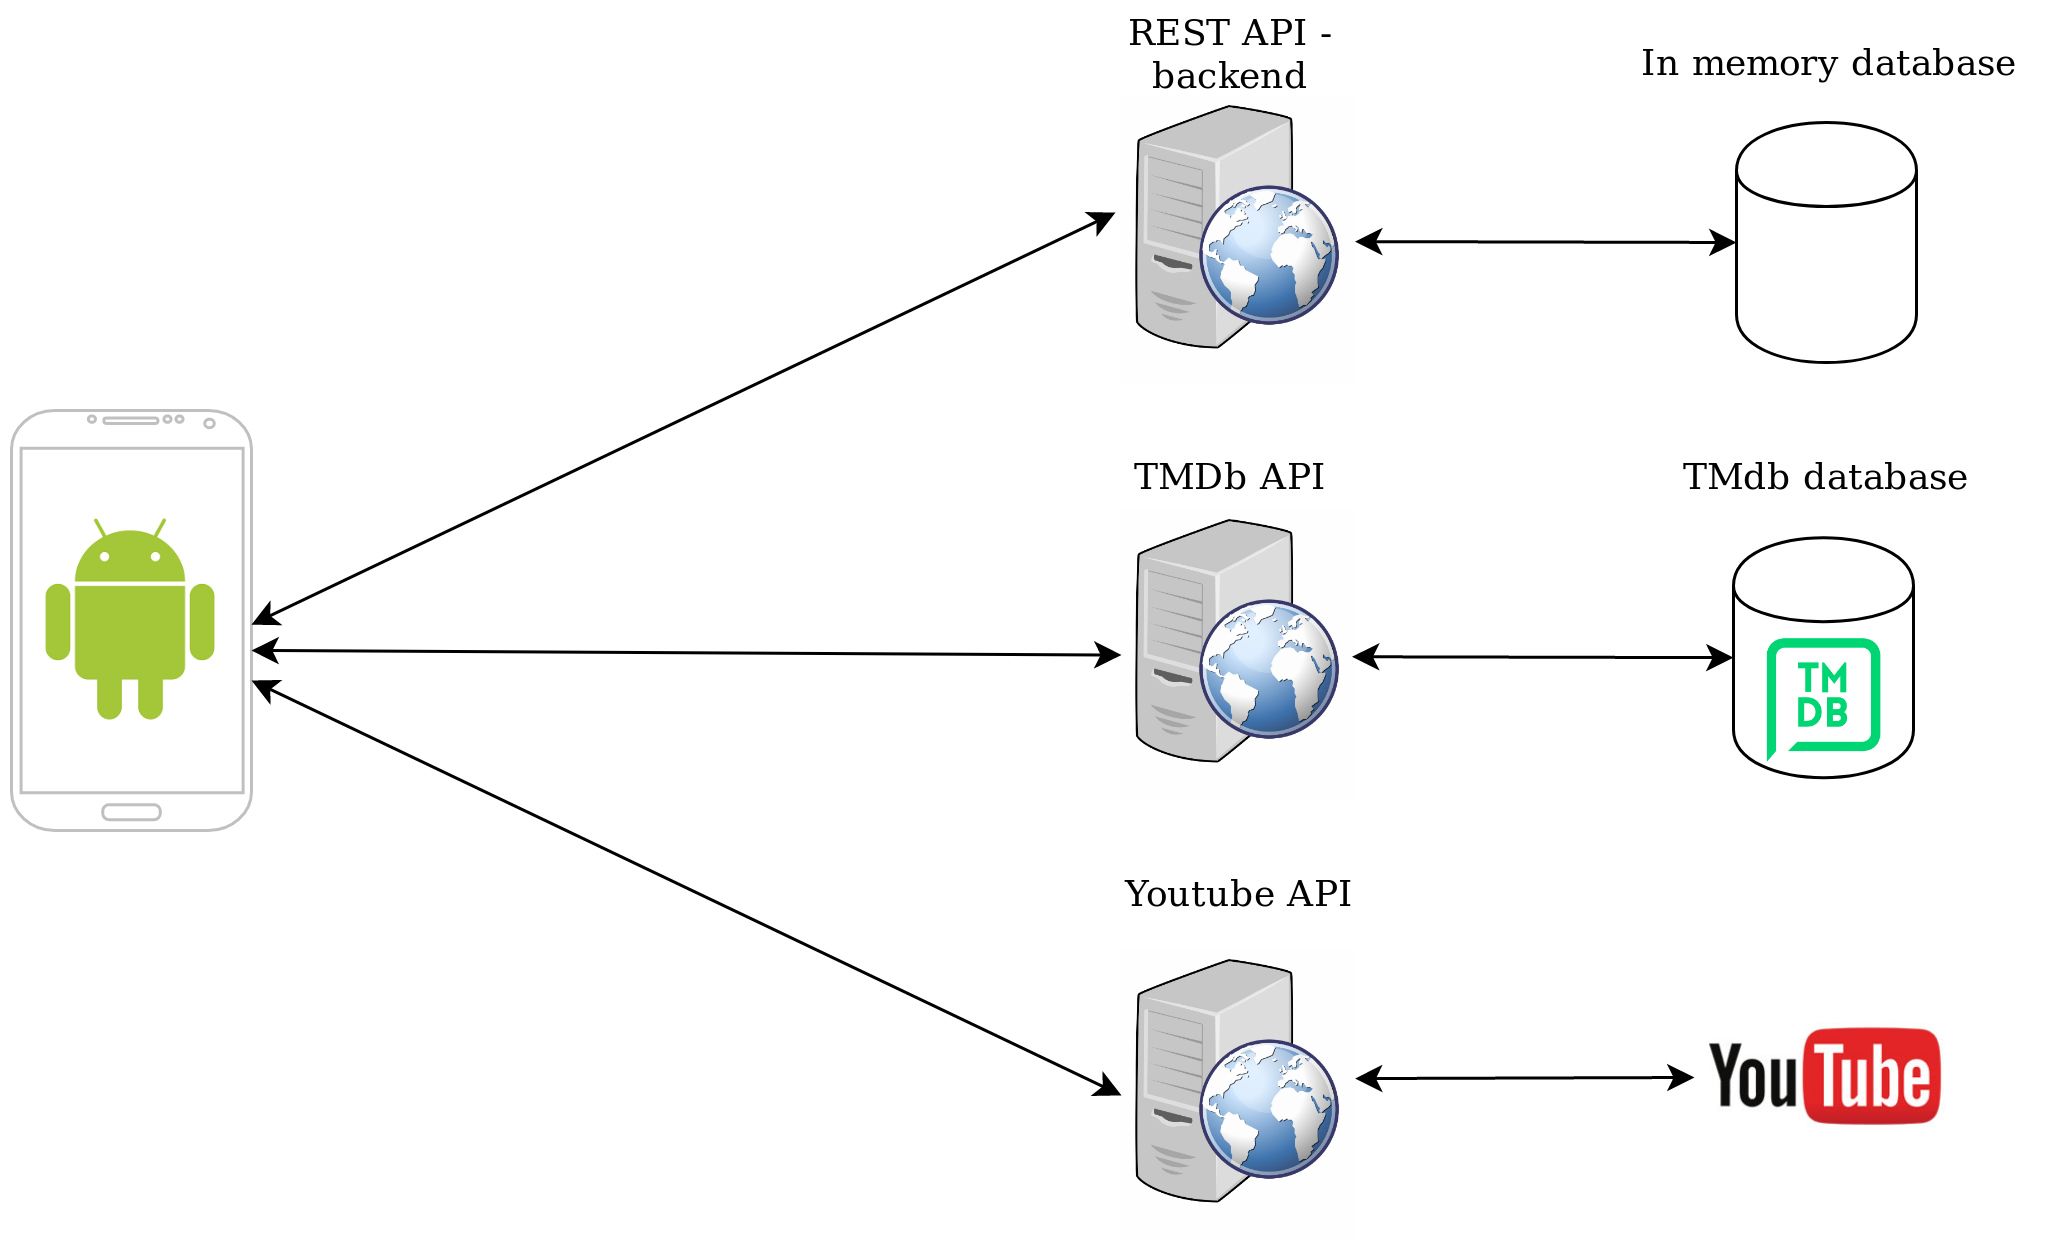
\includegraphics[width=0.8\textwidth]{img/schemas/APIs.png}
    \end{center}
    \caption{Usage des APIs}
    \label{apis_usage}
\end{figure}

\subsubsection{API TMDb}
L'\acrshort{api} principalement utilisée dans notre projet est celle proposée par \textit{The Movie Database} (TMDb) \cite{tmdb} qui offre toutes les informations sur les films et les acteurs. Nous avons également considéré \textit{The Open Movie Database} \cite{omdb}, mais elle offre beaucoup moins de possibilités. Nous interagissons avec cette \acrshort{api} en envoyant des requêtes HTTP en fonctions des besoins, nous recevons en retour les informations au format \acrshort{json}. La route GET : \mintinline{text}{/discover/movie} nous retournera les informations visibles au listing \ref{tmdb_example} au format \acrshort{json}.
\bigbreak
\begin{code}
    \begin{minted}[bgcolor=mygray,breaklines,breaksymbol=,linenos,frame=single,stepnumber=1,tabsize=2]{json}
{
  "page": 1,
  "total_results": 10000,
  "total_pages": 500,
  "results": [
    {
      "popularity": 533.832,
      "vote_count": 1707,
      "video": false,
      "poster_path": "/db32LaOibwEliAmSL2jjDF6oDdj.jpg",
      "id": 181812,
      "adult": false,
      "backdrop_path": "/jOzrELAzFxtMx2I4uDGHOotdfsS.jpg",
      "original_language": "en",
      "original_title": "Star Wars: The Rise of Skywalker",
      "genre_ids": [ 28, 12, 878 ],
      "title": "Star Wars: The Rise of Skywalker",
      "vote_average": 6.7,
      "overview": "The surviving Resistance faces the First Order ...",
      "release_date": "2019-12-18"
    },
    ...
  ]
    \end{minted}
    \caption{Exemple de données retournées par TMDb}
    \label{tmdb_example}
\end{code}
\bigbreak

\subsubsection{API REST Backend}
Certaines données de l'application nécessitent d'être persistées, c'est pourquoi nous avons choisi de mettre en place un backend basé sur Akka HTTP \cite{akka} en Scala. Le Scala est un langage relativement proche du Kotlin qui fait également usage de la \acrshort{jvm} et offre de nombreux atouts comme un typage fort, abstraction et programmation orientée objet, et permet d'écrire le code de manière simple, concise et déclarative. Pour toutes ces raisons, le choix de ce langage nous semblait judicieux. Les routes mises à disposition par cette API REST nous permettent de persister les informations telles que les comptes des utilisateurs, les relations d'abonnements entre eux et les appréciations des films. Elles permettent également de s'authentifier, s'enregistrer et rechercher un utilisateur.

\subsubsection{API YouTube}
Pour chaque film, TMDb nous offre une liste de vidéos YouTube, comprenant des \textit{trailers} et \textit{teasers} du film. Nous avons alors fait usage de l'\acrshort{api} officielle YouTube \cite{youtube} pour intégrer ces vidéos. Il faut obligatoirement créer une clé \acrshort{api} dans son compte Google pour pouvoir utiliser cette \acrshort{api}. On peut utiliser cette \acrshort{api} globalement de deux manières différentes sur Android :
\begin{itemize}
    \item \mintinline{text}{YouTubePlayerView} et \mintinline{text}{YouTubePlayerFragment} : offrent un plus grand contrôle sur la gestion de l'interface et des contrôles d'une vidéo ainsi que de son cycle de vie au prix de plus de code à écrire et à gérer.
    \item \mintinline{text}{YouTubeStandalonePlayer}: la manière plus simple et rapide d'utiliser l'\acrshort{api}, utilise l'application officielle YouTube. Le player attend l'identifiant d'une vidéo et la clé \acrshort{api} et démarre l'activité de l'application officielle YouTube.
\end{itemize}

Nous avons décidé d'utiliser la deuxième méthode car nous n'avons pas besoin d'un contrôle fin sur le lancement des vidéos. Pour chaque vidéo obtenue sur la vue des détails d'un film, nous commençons par récupérer un \textit{thumbnail} de chaque vidéo avec ce lien : \mintinline{text}{https://img.youtube.com/vi/$youtubeId/1.jpg}. Nous superposons ensuite une icône "play" et ajoutons un listener qui démarre la vidéo sur chaque \textit{thumbnail}. Un \mintinline{kotlin}{catch} de \mintinline{kotlin}{ActivityNotFoundException} est inclu avec affichage d'un message dans un "toast" dans le cas où l'utilisateur n'a pas l'application officielle YouTube installée sur son appareil.

\subsection{Fragments}
Toutes les vues de l'application sont implémentées à l'aide de fragments. Chaque fragment est associé à un layout (fichier \acrshort{xml}) qui décrit son aspect graphique. Le code Kotlin propre au fragment nous permet uniquement de définir une implémentation qui permet l'interaction entre les différents composants graphiques de la vue et la logique métier de l'application. Notre code est ainsi réutilisable dans plusieurs vues différentes.

\subsection{Single Activity}
Selon le cours et la documentation officielle d'Android \cite{docandroid}, l'architecture actuelle conseillée pour le développement d'une application repose sur le principe de n'utiliser qu'une seule activité composée de fragments, représentant les vues de l'application, illustré en figure \ref{single_activity}.
\begin{figure}
    \begin{center}
        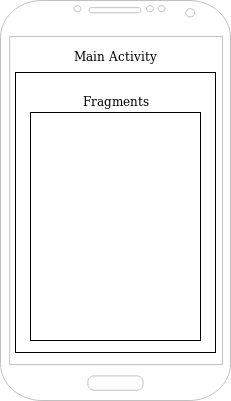
\includegraphics[width=0.5\textwidth]{img/schemas/Single_Activity.png}
    \end{center}
    \caption{Représentation d'une unique activité Android}
    \label{single_activity}
\end{figure}

\subsection{Navigation component}
Plusieurs possibilités s'offraient à nous concernant la navigation entre les différents fragments. Nous avons choisi d'expérimenter la nouvelle méthode proposée par la documentation officielle d'Android \cite{docandroid} qui est très intéressante et efficace.
Cette méthode repose sur un graphe de navigation qui est éditable graphiquement ou en \acrshort{xml}, comme illustré à la figure \ref{nav_graph}. Les noeuds de ce graphe sont les relations entre les différents fragments de l'application et les arcs symbolisent les actions de navigation d'un fragment à un autre avec des éventuelles données passées en arguments de ces actions. Ce composant de navigation génère ainsi le code des actions de navigation en fonction de ce qui a été décrit en \acrshort{xml}.
\begin{figure}
    \begin{center}
        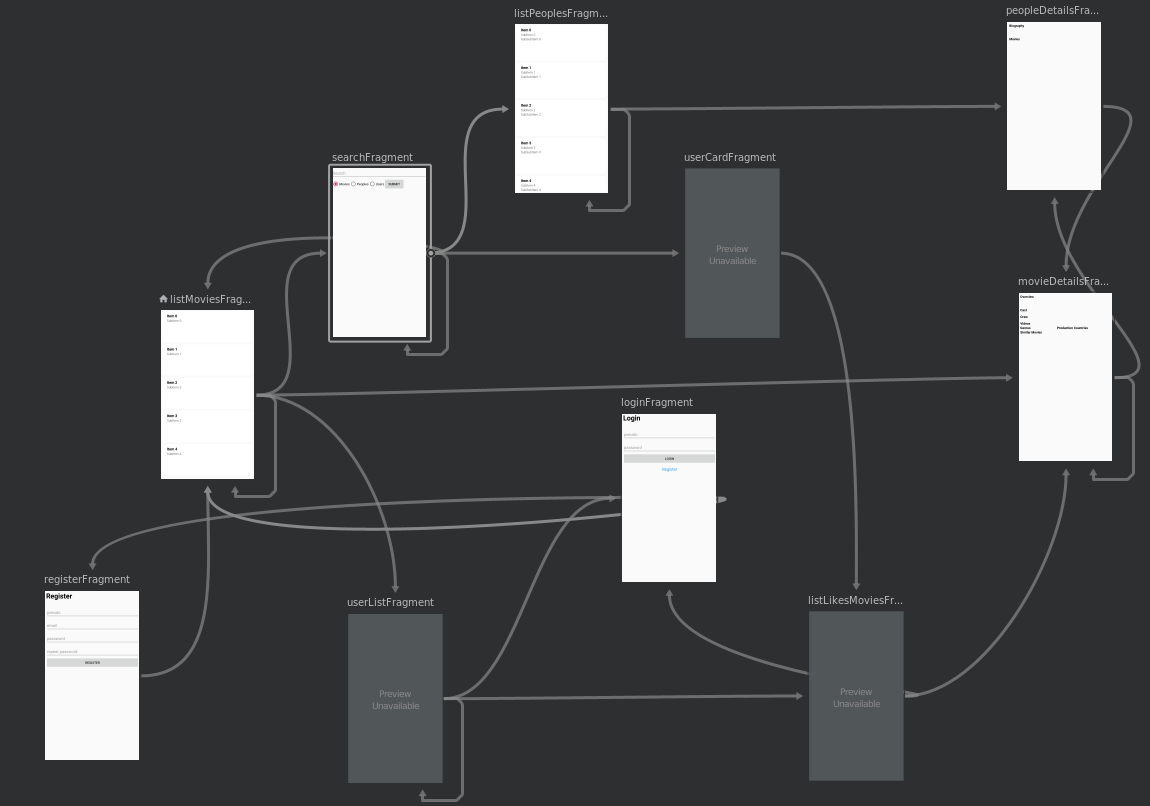
\includegraphics[width=1\textwidth]{img/screenshots/nav_graph.png}
    \end{center}
    \caption{Graphe de navigation de notre application}
    \label{nav_graph}
\end{figure}

Un exemple de code qui permet de naviguer de la liste des films vers les détails d'un film en utilisant cette classe générée automatiquement est disponible au listing de code \ref{nav_kotlin}.
\bigbreak
\begin{code}
    \begin{minted}[bgcolor=mygray,breaklines,breaksymbol=,linenos,frame=single,stepnumber=1,tabsize=2]{kotlin}
view.findNavController()
    .navigate(ListMoviesFragmentDirections
        .actionListMoviesFragmentToMovieDetailsFragment(item.id, item.urlImg))
    \end{minted}
    \caption{Exemple de navigation}
    \label{nav_kotlin}
\end{code}
\bigbreak


\subsubsection{Arguments}
Il est également possible de définir des arguments transmissibles entre fragments, la classe générée automatiquement prendra en compte ces derniers. Du côté du fragment qui sera appelé, une méthode très pratique est à disposition, permettant de réceptionner ces arguments, comme décrit dans le listing \ref{args_kotlin}.
\bigbreak
\begin{code}
    \begin{minted}[bgcolor=mygray,breaklines,breaksymbol=,linenos,frame=single,stepnumber=1,tabsize=2]{kotlin}
private val args: MovieDetailsFragmentArgs by navArgs()
movieId = args.id
urlImg = args.urlImg
    \end{minted}
    \caption{Arguments du graphe de navigation en Kotlin}
    \label{args_kotlin}
\end{code}
\bigbreak


\subsection{Volley}
\subsubsection{Généralités}
Notre application est majoritairement composée d'appels HTTP à diverses \acrshort{api}s. Nous avons utilisé la librairie Android conseillée dans la documentation officielle \cite{docandroid}, Volley \cite{volley}. Elle supporte nativement les requêtes sur des chaines de caractères bruts, des images ou du \acrshort{json}. Le listing \ref{volley_kotlin_simple} décrit un exemple d'utilisation : tout d'abord il faut instancier une queue de requêtes, ensuite définir deux \textit{callbacks} traitant les cas de réussite ou d'échec de la requête, enfin ajouter ces \textit{callbacks} à la queue de requêtes. Volley exécute ensuite les requêtes se trouvant dans la queue de manière asynchrone (sans bloquer le \textit{thread} principal d'affichage) et transparente pour l'utilisateur. Il est conseillé de déclarer une seule instance de Volley avec le \textit{pattern} singleton.
\bigbreak
\begin{code}
    \begin{minted}[bgcolor=mygray,breaklines,breaksymbol=,linenos,frame=single,stepnumber=1,tabsize=2]{kotlin}
val textView = findViewById<TextView>(R.id.text)
val queue = Volley.newRequestQueue(this)
val url = "http://www.google.com"
val stringRequest = StringRequest(Request.Method.GET, url,
        Response.Listener<String> { response ->
            textView.text = "Response is: ${response.toString()}"
        },
        Response.ErrorListener { textView.text = "That didn't work!" })
queue.add(stringRequest)
    \end{minted}
    \caption{Usage de la librairie Volley}
    \label{volley_kotlin_simple}
\end{code}
\bigbreak

\subsubsection{Asynchronisme}
Dans la majorité des cas, la logique de l'application requiert d'avoir reçu certaines informations en provenance des APIs avant de pouvoir les afficher sur la vue. Nous avons besoin de garantir que l'intégralité des données soient réceptionnées avant de les afficher, mais tout cela avec la contrainte de ne pas bloquer l'affichage.
Nous avons donc utilisé le mécanisme de fonctions de \textit{callback}. Le principe est simple, la fonction de \textit{callback} n'est appelée que lorsque la requête HTTP est effectué et les données réceptionnées. Un résumé de ce comportement est illustré à la figure \ref{asynchrone}.
\begin{figure}
    \begin{center}
        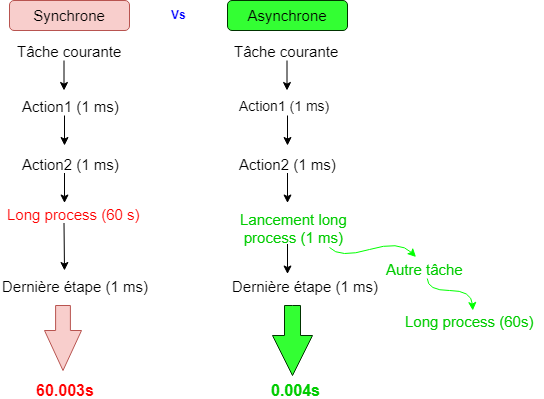
\includegraphics[width=0.8\textwidth]{img/schemas/Asynchronisme2.png}
    \end{center}
    \caption{Différences entre un fil d'exécution synchrone et asynchrone}
    \label{asynchrone}
\end{figure}

\subsubsection{Améliorations}
Etant donné le nombre d'appels HTTP important dans notre application, le code devient rapidement "pollué" par ce code long et répétitif de requête HTTP. Nous avons suivi les bonnes pratiques et simplifié cela en créant une classe \mintinline{text}{VolleyRequestController} offrant les méthodes relatives à tous les appels HTTP. Un exemple d'une requête HTTP GET utilisant cette classe est visible au listing \ref{volley_kotlin}. Nous avons également activé le cache réseau sur disque pour améliorer les performances d'affichage des vues.
\bigbreak
\begin{code}
    \begin{minted}[bgcolor=mygray,breaklines,breaksymbol=,linenos,frame=single,stepnumber=1,tabsize=2]{kotlin}
fun httpGet(URL: String, context: Context, callback: ServerCallback<JSONObject>) {
    val jsonObjReq = JsonObjectRequest(Request.Method.GET, URL, null,
    Response.Listener { response -> callback.onSuccess(response) },
    Response.ErrorListener { error ->
        Log.println(Log.DEBUG, this.javaClass.name, "error in httpGet : $error,\n$URL\n$callback")
    })
    HttpQueue.getInstance(context).addToRequestQueue(jsonObjReq)
}
    \end{minted}
    \caption{Usage de la librairie Volley avec \textit{callback}}
    \label{volley_kotlin}
\end{code}
\bigbreak

\subsubsection{Toolbar}
En haut de l'écran se trouve une barre comportant le nom du fragment courrant, un bouton "home" (\ref{films-tendance}) et un contrôle faisant apparaitre le menu latéral.

\subsection{Drawer}
Le drawer est un menu latéral qui apparaît de gauche à droite de l'écran. Ce menu permet d'afficher les informations relatives au profil de l'utilisateur courant. D'autre part, il propose les action de connexion, création de compte et déconnexion. Si l'utilisateur est connecté, il pourra aussi naviguer vers les vues des films aimés et du réseau d'amis.
Afin de rendre l'interface utilisateur plus conviviale, nous av
ons implémenté un \textit{drawer}, illustré à la figure \ref{drawer}. Ce \textit{drawer} repose également sur la dernière méthode proposée par la documentation d'Android \cite{docandroid}. L'interface graphique du \textit{drawer} est définie dans le \acrshort{xml} à l'aide d'un menu, et initialisée dans la \textit{main activity}. L'identifiant des différents items est nommé selon les identifiants référencés dans le graphe de navigation ce qui permet de naviguer directemnt vers le bon fragment lors de l'interaction d'un utilisateur avec ces derniers. Pour ce faire, le layout de la \textit{main activity} est de type \mintinline{text}{DrawerLayout}, elle inclut tout le contenu (\textit{top bar}, fragments de navigation, et \textit{bottom tabs}) ainsi que le \textit{drawer} qui sera affiché.
\begin{figure}
    \begin{center}
        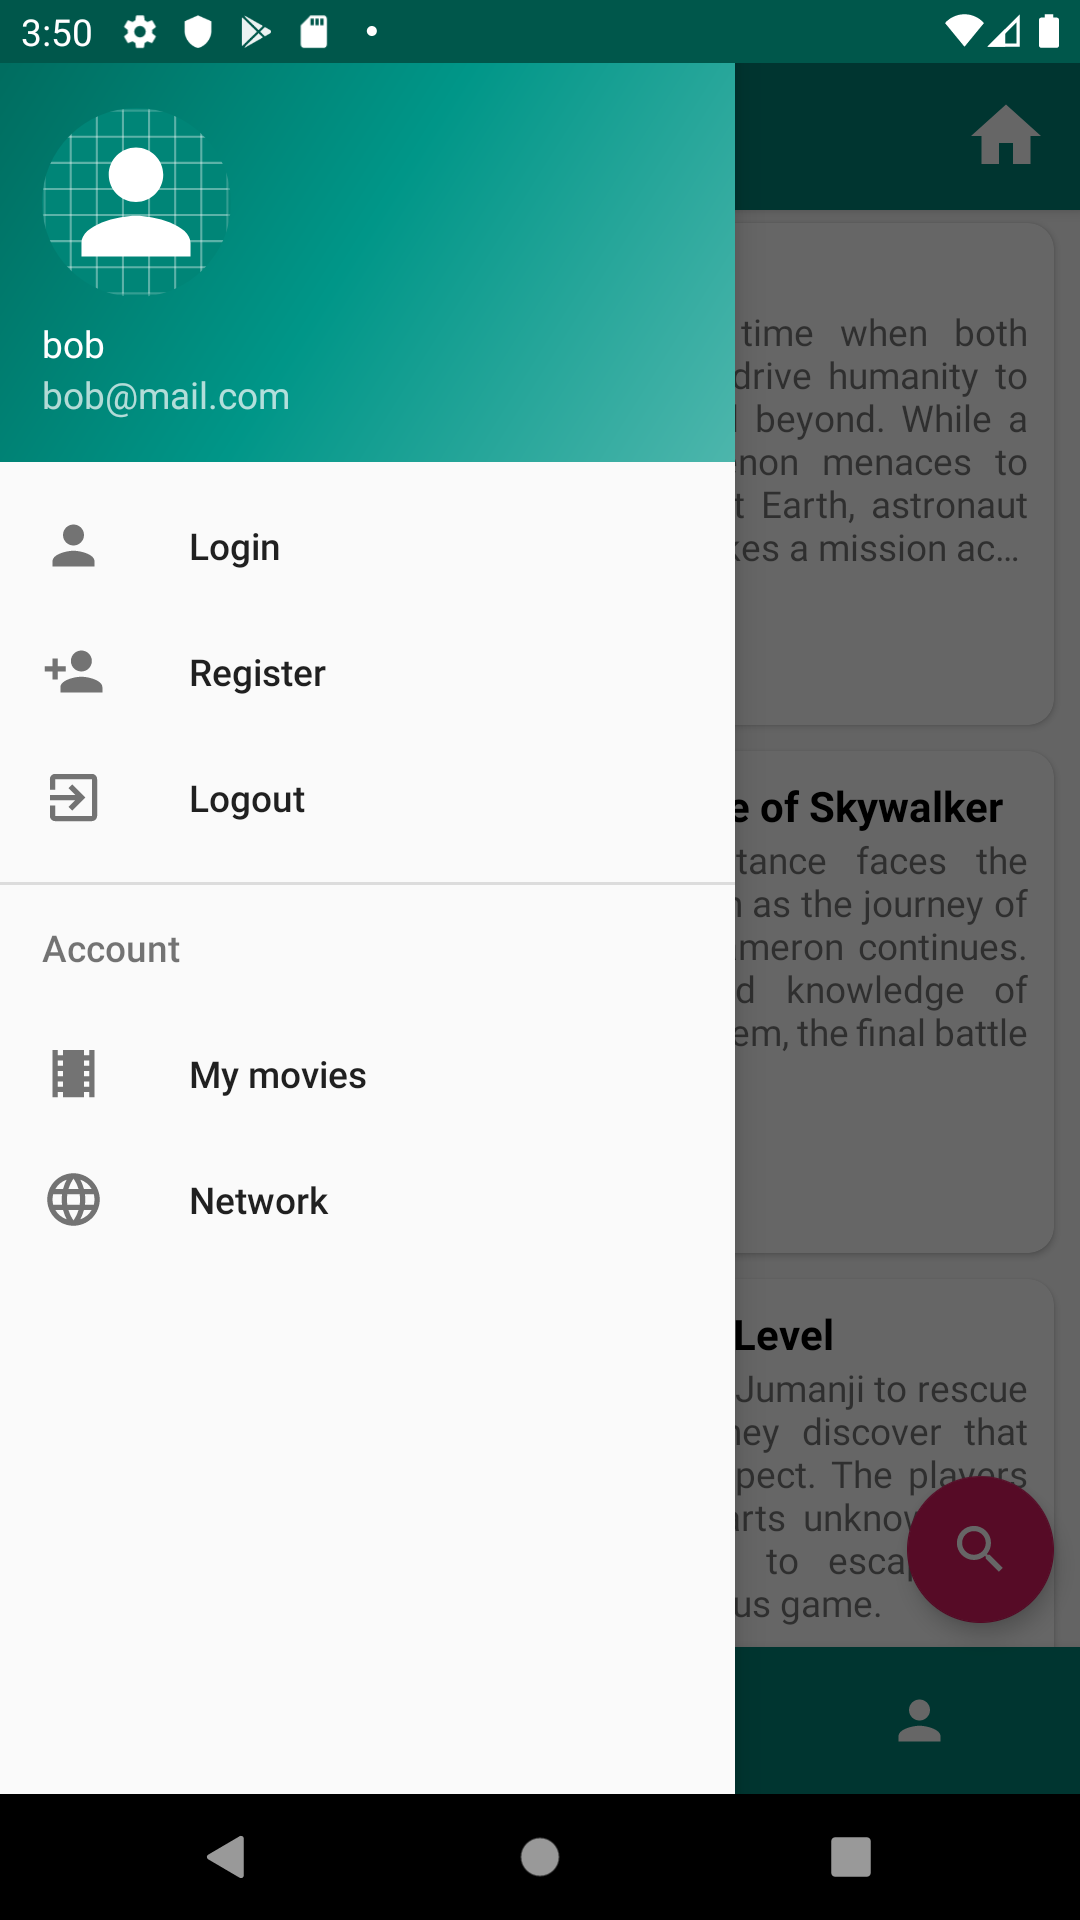
\includegraphics[width=0.5\textwidth]{img/screenshots/Drawer.png}
    \end{center}
    \caption{Drawer de l'application}
    \label{drawer}
\end{figure}

\subsection{Bottom tabs}
En bas de l'écran, des onglets de navigation sont présents, permettant de naviguer entre les vues principales de l'application, ces \textit{tabs} ont été implémentés à l'aide d'un menu classique Android défini au niveau \acrshort{xml}, illustrés à la figure \ref{tabs}. En basant l'identifiant de chaque item du menu sur les identifiants référencés dans le \textit{navigation graph}, chaque fragment est correctement appelé et affiché lors du clic sur un onglet.

\begin{figure}
    \begin{center}
        
\includegraphics[width=0.8\textwidth]{img/screenshots/Bottom_Tabs.png}
    \end{center}
    \caption{Onglets de l'application}
    \label{tabs}
\end{figure}

\subsection{View pager}

Pour les vues concernant les films appréciés/non appréciés et les utilisateurs suivis/abonnés, il était pratique de pouvoir passer d'une liste à l'autre rapidement et efficacement, comme illustré aux figures \ref{view_pager1} et \ref{view_pager2}. Nous avons donc mis en place des \textit{view pagers} qui sont en quelque sorte des sous-onglets permettant de "switcher" entre différents fragments assez rapidement. La réutilisation du code pour chaque sous-onglet (uniquement un changement de paramètre) est un avantage supplémentaire.
\begin{figure}
    \begin{center}
        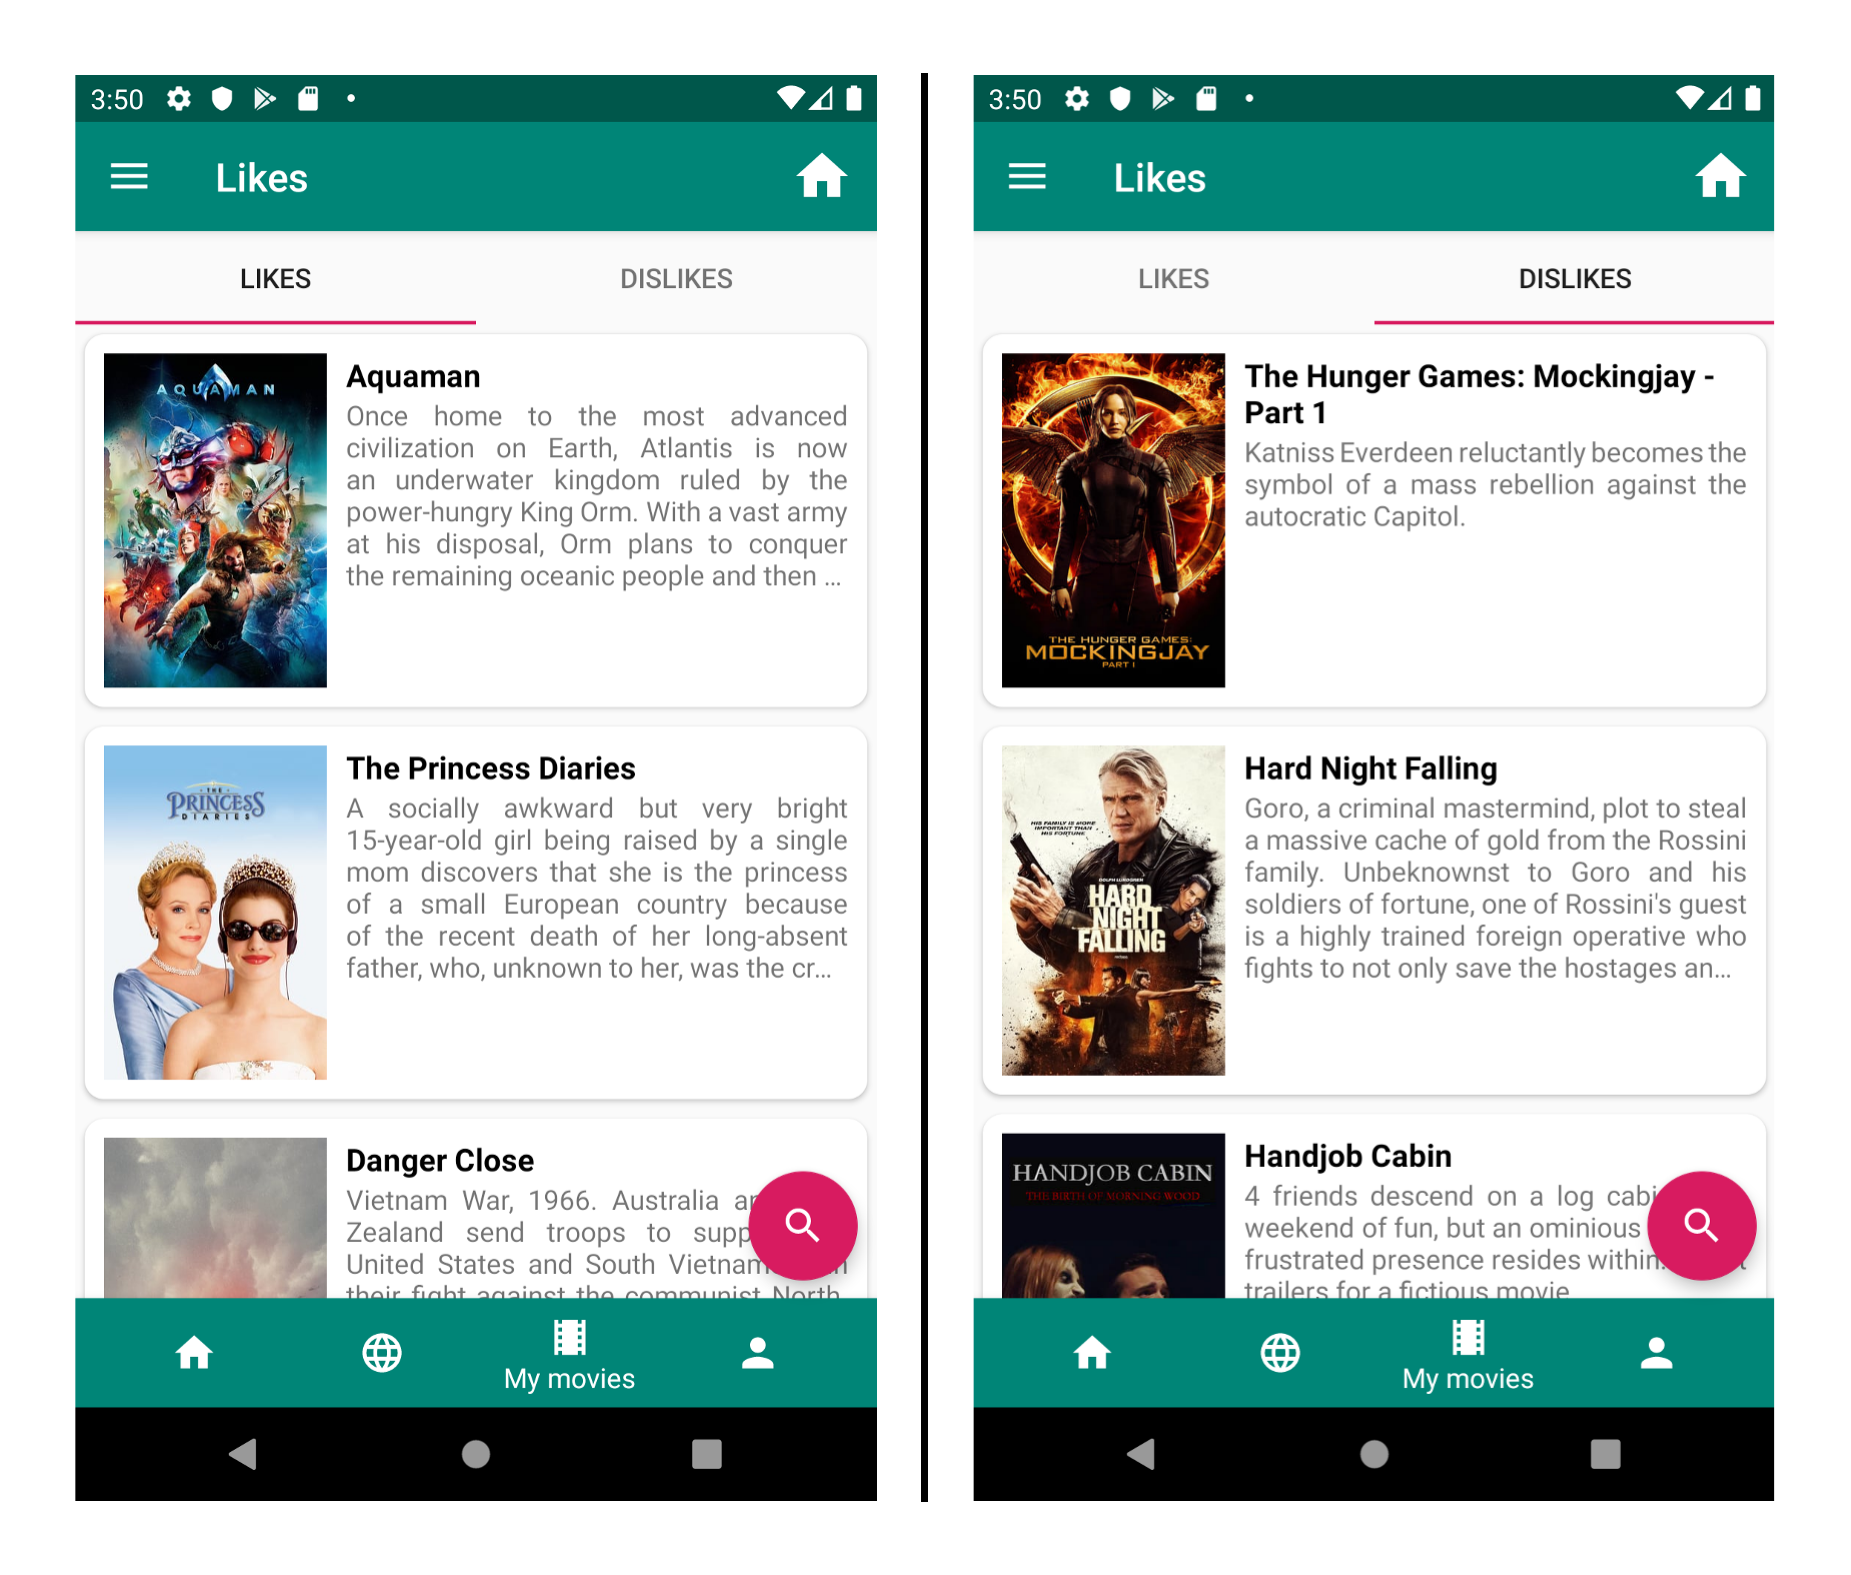
\includegraphics[width=0.8\textwidth]{img/screenshots/ViewPager1.png}
    \end{center}
    \caption{Appreciations des films dans l'application}
    \label{view_pager1}
\end{figure}

\begin{figure}
    \begin{center}
        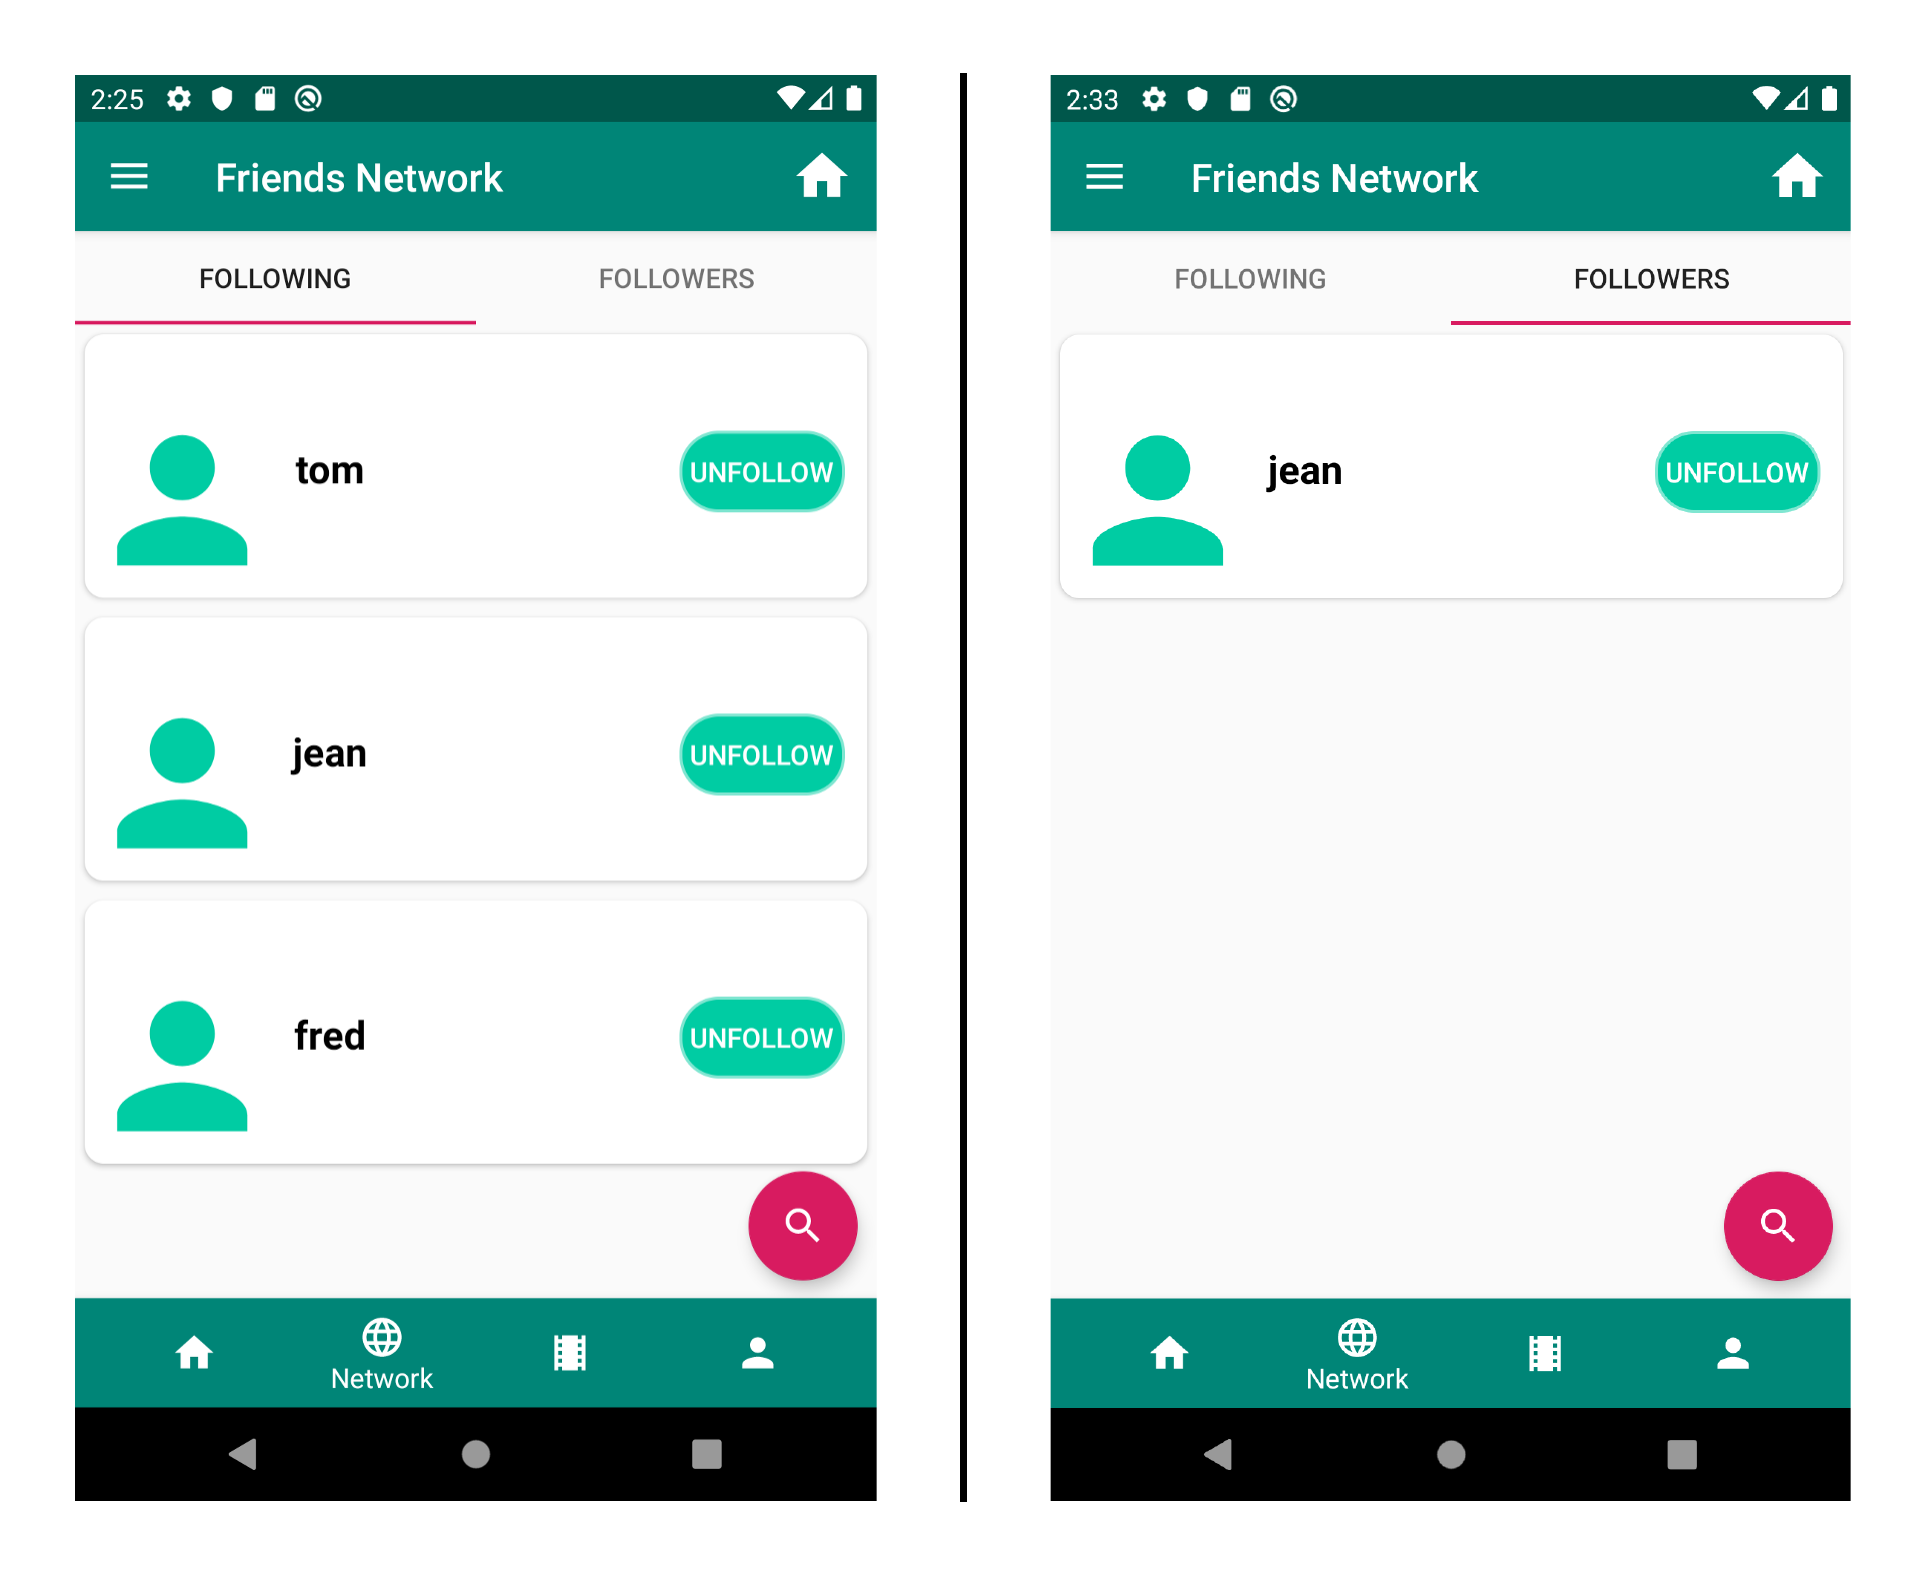
\includegraphics[width=0.8\textwidth]{img/screenshots/ViewPager2.png}
    \end{center}
    \caption{Réseau social dans l'application}
    \label{view_pager2}
\end{figure}

\subsection{Recherche}
La recherche est un fragment qui contient, au niveau \acrshort{xml}, uniquement un champ texte dans lequel les mots-clé sont saisis et un bouton radio sélectionnant dans quelle rubrique rechercher.
Lorsque l'action de recherche est effectuée, une \textit{recycler view} présentant les résutats de la recherche est affichée. La \textit{recycler view} appelée est toujours la même, nous avons uniquement le type des éléments affichés et le layout associé qui varient en fonction du type de la recherche (voir section \ref{generic-adapter}).
\begin{figure}
    \begin{center}
        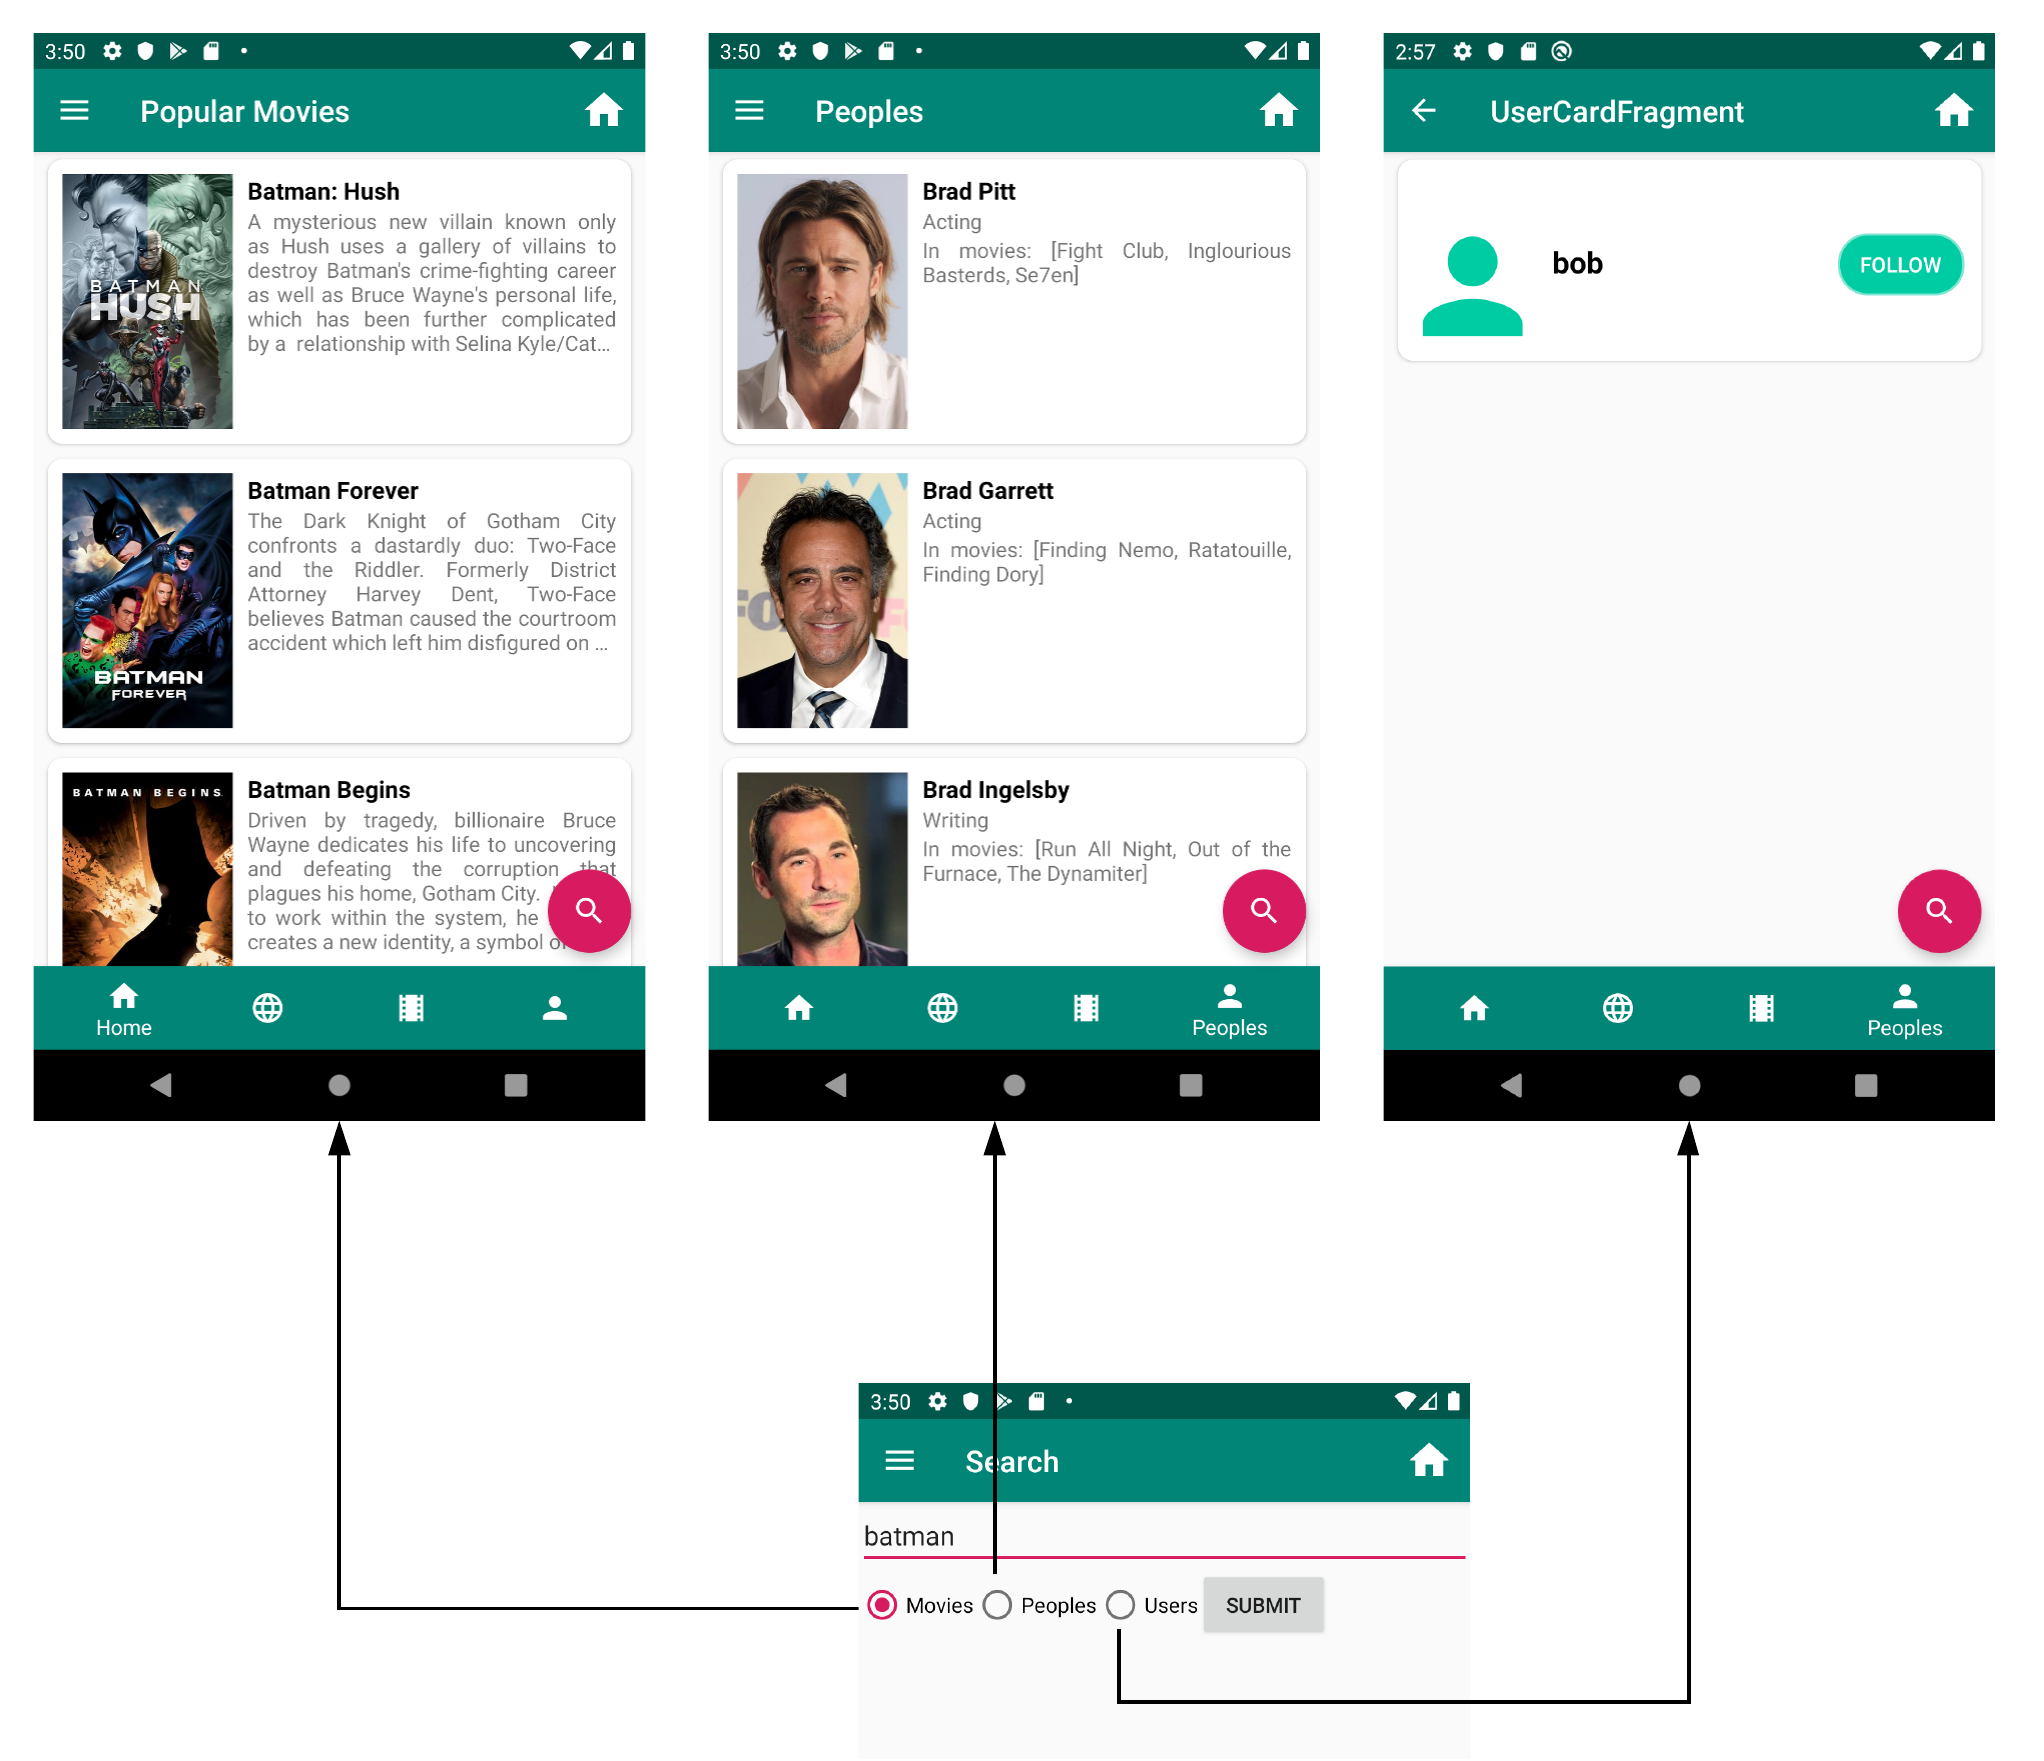
\includegraphics[width=1\textwidth]{img/schemas/Search.png}
    \end{center}
    \caption{Vue de la recherche dans l'application}
    \label{search}
\end{figure}


\subsection{Shared preferences}
Afin de stocker la session d'un utilisateur connecté à l'application, nous avons fait usage des \textit{shared preferences} qui sont un moyen simple (ensemble de clés-valeurs) et pratique de persister des information dans l'application et d'y accéder depuis les différents fragments. Deux exemples de leur utilisation sont disponibles aux listings \ref{share_prefs_kotlin1} et \ref{share_prefs_kotlin2}. Ce mécanisme permet également de vérifier qu'un utilisateur soit authentifié et de le rediriger vers la page de login dans le cas échéant.
\bigbreak
\begin{code}
    \begin{minted}[bgcolor=mygray,breaklines,breaksymbol=,linenos,frame=single,stepnumber=1,tabsize=2]{kotlin}
val sharedPref = activity?
    .getSharedPreferences(getString(R.string.preference_file_key), 
    Context.MODE_PRIVATE) ?: return
with (sharedPref!!.edit()) {
    putString(getString(R.string.pseudo), pseudo)
    putString(getString(R.string.email), email)
    putString(getString(R.string.token), token)
    commit()
}
    \end{minted}
    \caption{Création des \textit{shared preferences}}
    \label{share_prefs_kotlin1}
\end{code}
\bigbreak

\bigbreak
\begin{code}
    \begin{minted}[bgcolor=mygray,breaklines,breaksymbol=,linenos,frame=single,stepnumber=1,tabsize=2]{kotlin}
val auth = Common.getAuth((activity as MainActivity).
    getSharedPreferences(getString(R.string.preference_file_key),
    Context.MODE_PRIVATE), view.context)
if (auth != null) {
    ....
}
    \end{minted}
    \caption{Vérification des \textit{shared preferences}}
    \label{share_prefs_kotlin2}
\end{code}
\bigbreak

\subsection{FAB}
Un \textit{floating action button} (FAB) est disponible en bas à droite de l'écran, comme illustré dans la figure \ref{fab} un écouteur sur ce bouton est défini dans la \textit{main activity} permettant d'intercepter les interactions des utilisateurs. Lorsqu'une interaction est détectée, une redirection vers le fragment dédié à la recherche est effectuée.
\begin{figure}
    \begin{center}
        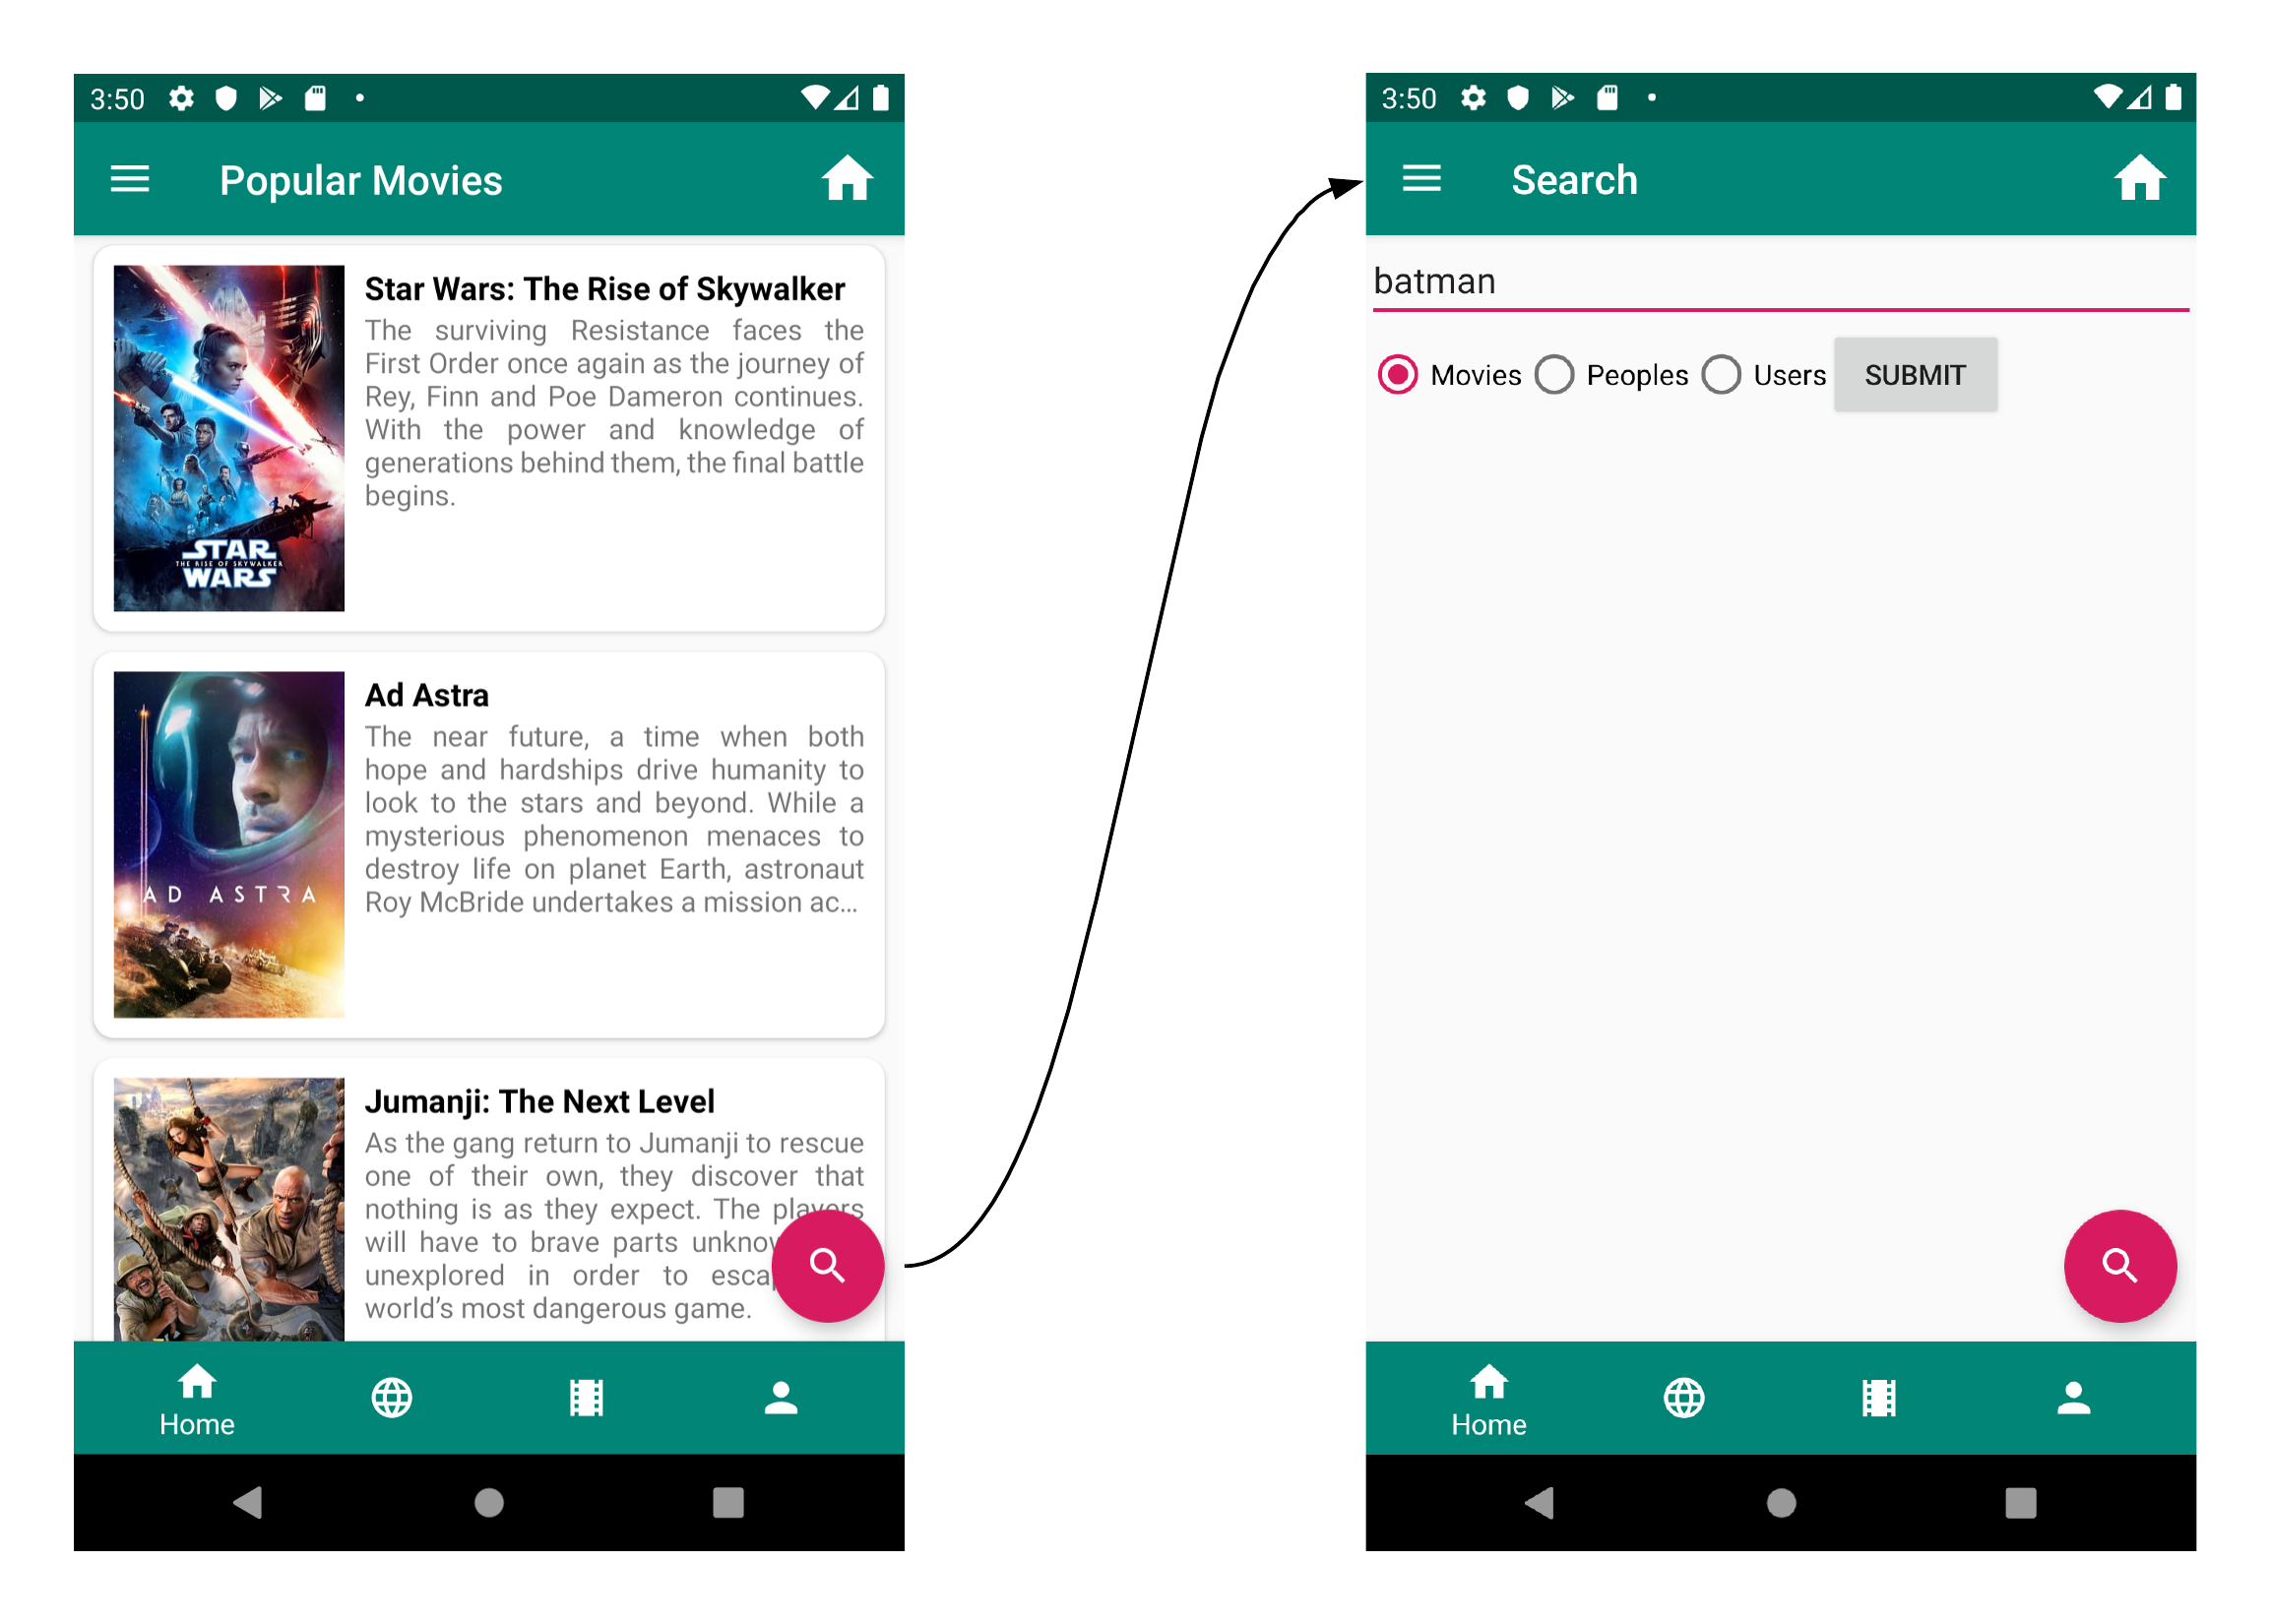
\includegraphics[width=0.8\textwidth]{img/screenshots/FAB.png}
    \end{center}
    \caption{FAB de l'application}
    \label{fab}
\end{figure}

\subsection{Generic adapter}\label{generic-adapter}
Dans le cadre de cette application, nous travaillons très fréquemment avec la \textit{recycler view} qui affiche une liste d'items, d'un même type pour toute la liste. Afin de ne pas devoir recréer une \textit{recycler view} par type d'items, nous avons choisi d'implémenter un adapteur générique permettant de réutiliser la même liste mais avec des items de type différents, comme illustré à la figure \ref{generic_adapter_img}.
\begin{figure}
    \begin{center}
        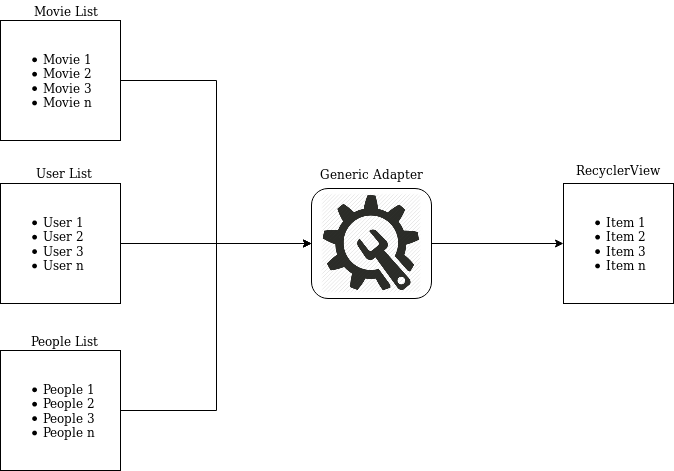
\includegraphics[width=0.8\textwidth]{img/schemas/Generic_Adapter.png}
    \end{center}
    \caption{Principes de l'adapteur générique}
    \label{generic_adapter_img}
\end{figure}
\newpage

\section{Conclusion} %-----------------------------------------------------------------------------------------------
\subsection{Bilan personnel}
Pour conclure, ce projet nous a permis d'apprendre et mettre en pratique de nombreux concepts propres à la programmation Android. Nous nous sommes également familiarisé avec le langage Kotlin, qui, une fois pris en main, simplifie et optimise grandement les opérations qui peuvent être plus complexes et fastidieuses en Java. Enfin, nous restons sur un sentiment très satisfaisant de cette première expérience dans le monde du développement Android.

\subsection{Problèmes rencontrés}
Les principales difficultés rencontrées durant le développement de ce projet sont les suivantes :
\begin{itemize}
    \item Prise en main de la documentation Android officielle : par moments des raccourcis sont pris dans les explications, les morceaus de code fournis ne sont pas forcément entiers. Nous pensons que les rédacteurs partent du principe que le lecteur a fait une lecture linéaire et dans l'ordre, chose que nous n'avons pas fait.
\end{itemize}

\subsection{Améliorations}
Les améliorations suivantes pourraient être apportées au projet :
\begin{itemize}
    \item L'interface graphique qui est toujours optimisable.
    \item La mise en place d'un cache qui éviterait de réinterroger l'API pour chaque action effectuée et par conséquent limiter le traffic réseau.
    \item Interrogation de l'API Netflix afin de savoir si le film est disponible sur leur plateforme de streaming.
    \item Afficher les films à la une en fonction des préférences de l'utilisateur, par exemple déduites de ses films appréciés ou de ses recherches récentes.
    \item Afficher les informations relatives aux horaires des cinémas les plus proches pour les films actuellement dans les salles.
    \item Notifier les utilisateurs lorsqu'ils sont suivis par un autre utilisateur.
    \item Gestion de plusieurs langues.
\end{itemize}

\newpage

\section{Références} %-----------------------------------------------------------------------------------------------
\bibliographystyle{unsrt}
\bibliography{bib}

\end{document}

% \begin{figure}
%     \begin{center}
%         \includegraphics[width=0.8\textwidth]{images/image.png}
%     \end{center}
%     \caption{légende}
%     \label{label}
% \end{figure}

% \bigbreak
% \begin{code}
%     \begin{minted}[bgcolor=mygray,breaklines,breaksymbol=,linenos,frame=single,stepnumber=1,tabsize=2]{rust}
% fn main() {
%     println!("Hello, world!");
% }
%     \end{minted}
%     \caption{Hello world en Rust}
%     \label{label}
% \end{code}
% \bigbreak

% \bigbreak
% \begin{code}
%     \inputminted[bgcolor=mygray,breaklines,breaksymbol=,linenos,frame=single,stepnumber=1,
%         tabsize=2,firstline=157,lastline=185]{rust}{file.rs}
%     \caption{légende}
%     \label{label}
% \end{code}
% \bigbreak
